\documentclass[twoside]{uva-inf-bachelor-thesis}
%\usepackage[dutch]{babel}

% Filling your thesis with only lorem ipsum is not advised.
\usepackage{lipsum}
%for highlighting findings
\usepackage{tcolorbox}
\usepackage[style=numeric-comp]{biblatex}
\usepackage{cleveref}
\usepackage{todonotes}
\addbibresource{bib.bib}

% Title Page
\title{Mutation testing: ``Clustered'' and ``Contextual Predictive'' approaches analysed}
\author{Adam Abdalla}
\supervisors{Ana Oprescu, PhD.}
\signedby{Signees}

\begin{document}
\maketitle

\begin{abstract}
Many software projects require test suites to ensure changes do not negatively affect the project. However, test suites are not always foolproof. This issue has brought rise to the idea of mutation testing. However, the time cost of mutation testing is far too large for it to be viable in practice. Several solutions have been proposed by state-of-the-art work, including ``Clustered Mutation Testing'', or ``CMT'' for short. Previous students at the University of Amsterdam have implemented clustered mutation testing and analysed its performance regarding its ability to imitate the results of full mutation testing.

This thesis consists of three parts. The first part inspects the speedup CMT creates over full mutation testing under varying circumstances. The second part discusses and tests potential improvements to the algorithm for the sake of bettering its ability to imitate full mutation testing. The last part introduces a novel algorithm, also discussing the implementation and performance thereof. 

Our first part reveals that CMT creates a significant speedup, although not in the same order as the state-of-the-art work. In our second part, we have also improved CMT's precision with the use of more rigorous pre-processing. Other changes to the algorithm were less fruitful. Lastly, our novel algorithm outperforms CMT in some cases, but not yet in general. Still, there is still a lot to be explored as far as potential improvements to this novel algorithm are concerned. We hope that this research will serve as a step towards making mutation testing viable for commercial use.
\end{abstract}

\tableofcontents

\chapter{Introduction}
Software engineering is often done under a lot of time pressure. For this reason, bigger projects will want to automate as much of the process as possible. Because it is usually a very repetitive part of the process, testing is ordinarily automated through the employment of test suites.

However, it is of the utmost importance for a lot of software projects that testing is done robustly, and manually created test suites regularly fail to do so. To combat this, methods to ensure robust test suites have been heavily discussed for decades~\cite{Harrold00}. This includes a wide array of approaches such as the systematic and automated creation of test suites~\cite{Fraser13}.

The approach we are focusing on in this thesis is ``mutation testing''~\cite{Jia11}. In this approach, test suites themselves are put to the test using a type of brute force attack. From a correct program, mutations are generated and given to the test suite. The number of mutants that remain uncaught by the end of the test suite is a good indicator of how robust that test suite is. Furthermore, a more detailed analysis of the weaknesses of a suite can be done by observing exactly which mutations passed through.

Although mutation testing certainly can ensure the creation of a robust test suite, it remains largely unused in practice despite the fact that the concept has existed for decades~\cite{Jia11}. This is because the time cost of testing all mutants with the test suite is too expensive.

Multiple innovations have been proposed and implemented in order to improve the time cost while keeping the test suite testing capability cost at a minimum~\cite{Zhang16, Basarat21}. One such innovation has been introduced by a student at the University of Amsterdam~\cite{Basarat21}. Based on the idea that mutants which share certain properties are also likely to share the same fate, he suggested clustering the mutants and only executing a singular mutant from each cluster. If the clusters are accurate enough, the result of testing that representative mutant can be seen as the result of each other mutant in the cluster with reasonable certainty. We will refer to this as ``Clustered Mutation Testing'', or ``CMT'' for short.

Another student, \textcite{Mouissie22}, has since expanded on the work of \textcite{Basarat21}, comparing the testing capabilities of CMT with different clustering algorithms, using both the ``weighted mutation score'' metric of \textcite{Basarat21} and his own ``cluster accuracy'' metric.

\section{Problem statement}
\textcite{Basarat21} and \textcite{Mouissie22} have thoroughly explored the accuracy cost of clustering. Although keeping as much of the testing capabilities of the full mutation testing is indeed something we are interested in when discussing these possible solutions to the issue of mutation testing. We are also interested in the time cost improvement. Therefore, this research starts with an examination of the time costs of mutation clustering.

Aside from assessing the time costs, improvements to the algorithm of mutation clustering will be sought out in order to enhance its accuracy.

Lastly, this research discusses, implements and tests a novel algorithm, which draws inspiration from CMT.

\section{Research questions}
For the time cost analysis, we look at the time cost of a complete run of CMT using the clustering algorithm originally used by \textcite{Basarat21}, namely Agglomerative clustering. Along with this, we inspect the time cost of another accurate algorithm of \textcite{Mouissie22}. For this, we have chosen Mean-shift, as it scores best in the average cluster accuracy. We compare these with the time cost of normal mutation testing since our original goal is to speed up that process. This leads to the following research questions:\\
\textbf{Research question 1:} How does hierarchical clustering mutation testing compare to clusterless mutation testing in terms of speed?\\
\textbf{Research question 2:} How does Mean-shift clustering mutation testing compare to clusterless mutation testing in terms of speed?

Once the time cost analysis of the clustered mutation testing process is completed, we can move on to enhancing its accuracy. Thus, our next question:\\
\textbf{Research question 3:} How can we make improvements to the accuracy performance of clustered mutation testing?

In its current form, clustered mutation testing takes only one thing into account when predicting the result of some mutant. Namely, the result of the most similar mutant that was tested. According to the results of \textcite{Basarat21}, this seems to be a powerful indicator. However, relying solely on that creates a ceiling for clustered mutation testing. Therefore, our final research question is:\\
\textbf{Research question 4:} How can we create a different algorithm that creates a new avenue for approximating the results of mutation testing?\\

\section{Contributions:}
The contributions of our research are the following:
\begin{itemize}
    \item A time cost comparison between full mutation testing and Clustered Mutation Testing using hierarchical clustering.
    \item A time cost comparison between full mutation testing and Clustered Mutation Testing using Mean-shift clustering.
    \item A slight improvement to the Clustered Mutation Testing algorithm provided by \textcite{Basarat21}.
    \item A new algorithm that may act as a foundation for an algorithm that outperforms Clustered Mutation Testing.
\end{itemize}

\section{Outline}
In \cref{chap:2} we address the background knowledge required for an easy understanding of the following chapters. \Cref{chap:3} discusses the time analysis part of the thesis, pertaining to research questions one and two. \Cref{chap:4} and \cref{chap:5} discuss the improvements made to Clustered Mutation Testing and the novel algorithm.
\Cref{chap:6} is an overall discussion, reflecting on the research as a whole and talking about the way forward.

\chapter{Theoretical background}
\label{chap:2}
This theoretical background is structured for the sake of the narrative. As such, the sections are not ordered in terms of importance. We annotated each section's header to indicate which chapter(s) it is important for. Vital for an easier understanding of this thesis are sections: 2.2 $\|$ 2.2.1 $\|$ 2.2.2 $\|$ 2.4 $\|$ 2.6.3.

\section{Mutation testing}
In mutation testing, a correct working program is slightly modified in many different ways. This is done by using a set of mutators, which seek a type of object, identifier, or pattern within the original code and change it. An example mutator is the Arithmetic Operator Replacement, which exchanges all arithmetic operations with different ones, with each exchange leading to a separate mutation~\cite{Mouissie22}. In modern mutation systems, some timing improvements which do not affect testing capabilities have already been implemented. For example, mutations that function the same as other mutations or the original program are removed~\cite{Beller21}. Well-known mutation testing tools for Java include MuJava and Major~\cite{muJava, major}. \textcite{Basarat21} considered these mutation testing tools.

However, he cites several ways in which they are worse than PIT~\cite{pit} from other papers. Alongside this, they lacked support for state-of-the-art testing tools. There may have been updates to MuJava and Major, there may also be a new mutation testing tool recently developed. Still, for our thesis, we have made the decision to continue using PIT. This is partially because the reasons provided by \textcite{Basarat21} make PIT seem like a project kept up-to-date with the state-of-the-art, but the bigger reason behind our decision is because we will be using the ``Pitest Clustering Plugin'' developed by \textcite{Basarat21}. This also means that our projects will remain java projects.

\subsubsection{Pitest Clustering Plugin, \textbf{\cref{chap:3}}}
Pitest offers great flexibility with its plugin system. Pitest works in multiple phases. During each of these phases, Pitest runs a basic script which can be replaced with plugin scripts~\cite{pitAdvanced}. These plugin scripts can change the functionality of Pitest very drastically. For example, Pitest can be given a list of certain mutations and run only those mutations. \textcite{Basarat21} has created the ``Pitest Clustering Plugin'' which contains a few different functionalities.

\begin{itemize}
    \item \textbf{Similarity}: calculates the Levenshtein distance between each mutation and the original class it was based on.
    \item \textbf{Characteristics}: Gathers various characteristics of the mutation.
    \item \textbf{Clustering}: Reads a csv of mutation - cluster pairs from a certain folder, picks only 1 mutation of each cluster at random and executes all picked mutations.
    \item \textbf{Report}: Consists of two scripts, one which reports the final status of each mutant and the number of tests it has undergone and one which reports the number of clusters killed with the clustering plugin and the total amount of clusters.
\end{itemize}

Each of these functionalities writes its output to files so we may draw analysis on them. We have also added a usage guide in the ``readme'' of the github of this project~\cite{aAbdalla-repo}.

\section{Identifying characteristics, \textbf{\cref{chap:4}, \cref{chap:5}}}
Pitest saves some metadata of each mutant during its creation. CMT uses this metadata to cluster mutants together. We will refer to this metadata as the characteristics of a mutant. One of our potential improvements in \cref{chap:4} discusses the pre-processing of these characteristics. We have also used these characteristics in our own algorithm in \cref{chap:5}. The characteristics used in this thesis are:
\begin{itemize}
    \item \textbf{Mutant Identifier}: A mixture of other characteristics resulting in a unique identifier of each mutant.
    \item \textbf{Mutant Operator}: Mutator employed by Pitest to create the mutant.
    \item \textbf{Opcode}: The original opcode that was changed by the mutator.
    \item \textbf{Return type}: The return statement contained by the mutant, a default value if there is no return statement.
    \item \textbf{In try-catch}: A binary value indicating whether or not the mutant is inside a try-catch block. 
    \item \textbf{Local variable count}: The number of local variables present at the mutant location.
    \item \textbf{Class name}: The name of the class the mutant is in.
    \item \textbf{Method name}: The name of the method the mutant is in.
    \item \textbf{Line number}: The line number the mutant is at.
\end{itemize}

\subsection{Characteristic categories, \textbf{\cref{chap:5}}}
Each of these characteristics has its own value. In \cref{chap:5}, we will be transforming the characteristics, so that every characteristic is a categorical variable. That means that every value of every characteristic is a ``category''.

\subsection{pk-score, \textbf{\cref{chap:5}}}
A vital part of the algorithm we introduce in chapter 5 is the ``percentage killed score'', or ``pk-score'' for short. The pk-score is calculated per characteristic category. The formula is as follows:
 \[p = k/t\]

Where:
\begin{itemize}
    \item p = pk-score of category
    \item t = total number of mutants, possessing the target category, tested
    \item k = number of mutants, possessing the target category, killed out of the tested ones
\end{itemize}

\subsection{Encoding,\textbf{\cref{chap:4}, \cref{chap:5}}}
To change categorical data into continuous data we used encoding. We used two different types of encoding: ``label-encoding'' and ``one-hot-encoding''. Label-encoding changes every possible category into a number, starting from one. One-hot-encoding changes every possible category into a separate column, where a binary value denotes whether or not the row is a part of the category.

\subsection{Locality, \textbf{\cref{chap:4}, \cref{chap:5}}}
The class name, method name and line number all indicate where the mutant is located. Only when used in combination, do they truly define where the mutant is. For this reason, we have combined them into a new characteristic: ``Locality''. An explanation of how exactly this is done is given in \cref{chap:4}, section 1.2.

\section{Hyperopt's fmin, \textbf{\cref{chap:4}, \cref{chap:5}}}
Hyperopt's fmin function takes an “objective” function and tries to minimize its return value. It does so by taking a list of input parameters for the objective function with their respective search spaces. It then runs the objective function with different input parameters selected from their search ranges each time. The fmin function returns a selection of input parameters which it predicts to be the best possible selection.

\section{Overhead, \textbf{\cref{chap:4}, \cref{chap:5}}}
The algorithms discussed in this thesis can be split into three phases:
\begin{itemize}
    \item The selection of the mutants to be tested
    \item The testing of the mutants using Pitest
    \item The processing of the results and prediction made based thereon
\end{itemize}
When we mention the term ``overhead'' while discussing an algorithm, we are referring to the first and third phases combined.

\section{Clustering Algorithms}
Clustering algorithms seek to discover natural groupings in data. There exists no such thing as ``the best clustering algorithm''. Each algorithm puts forward different strengths and weaknesses to suit a specific type of problem. For example, soft clustering algorithms result in data points being part of multiple clusters. This can be good for problems which require the confidence in the conclusions to be noted. However, a drawback of soft clustering algorithms is that they are usually slower. \textcite{Basarat21} and \textcite{Mouissie22} have considered various clustering algorithms to fit our data and interests.

\subsection{Hierarchical, \textbf{\cref{chap:3}}}
The first algorithm we are going to use is hierarchical clustering. Specifically Sklearn's ``AgglomerativeClustering''. Agglomerative clustering differs from its counterpart within hierarchical clustering in that it clusters from the bottom up. In other words, every data point becomes its own cluster. it then takes the two clusters with the least distance and merges them. This continues until the specified number of clusters is reached. By default, the distance is based on the total euclidean distance of all data points in the compared clusters. \textcite{Basarat21}  opted to use the ``ward'' linkage method, which merges clusters in a way which minimizes the variance of clusters being merged.~\cite{agglomerativeClustering} 

\subsection{Mean-shift, \textbf{\cref{chap:3}}}
The second algorithm we have decided to analyse CMT with is Sklearn's ``Mean-shift''. We have chosen this because it outperformed the other algorithms in the ``Clustering Accuracy'' metric in \textcite{Mouissie22}. On top of this, the computation requirements for the algorithm are high, so it may show whether or not spending a lot of computation time on clustering is an issue for the speed of the entire clustered mutation testing. In mean shift, each data point will iteratively move towards the most data point-dense region within a certain distance of the data point. The ``bandwidth'' parameter decides what that certain distance is. A lower bandwidth will lead to more clusters. With the ``cluster\_all'' parameter set to true, data points which do not have any other data points within the distance dictated by bandwidth will be added to the closest cluster at the end.

\subsection{KMeans, \textbf{\cref{chap:4}}}
In \cref{chap:4}, section 1.1, we switch to Sklearn's ``KMeans'', because it has a function that fits our needs. A basic KMeans algorithm works in iterations. A parameter-specified number of ``centroids'' are placed in random places in the dataset. Every iteration thereafter consists of two steps:
\begin{itemize}
    \item Each data point is assigned to a centroid based on its distance.
    \item The centroid is then moved to the center of its assigned data points.
\end{itemize}
The algorithm decides based on given parameters.

\subsection{Kmeans1d, \textbf{\cref{chap:5}}}
In \cref{chap:5}, we transform certain characteristics into categorical variables. We do this by clustering them and using the resulting cluster IDs as categories. Since the characteristics are all 1-dimensional values, we use a Kmeans implementation optimized for 1-dimensional clustering~\cite{kmeans1d}.

\section{Metrics}
\subsection{Weighted mutation score}
Both preceding studies used the ``weighted mutation score'' metric~\cite{Basarat21}. In full mutation testing, the mutation score refers to the number of mutations killed over the total number of mutants generated, generally conveyed in percentages. In clustered mutation testing, it is our goal to approximate the results of full mutation testing in less time. Clustered mutation testing does not give us the number of mutations that would be killed through full mutation testing. Thus, we instead approximate this by multiplying the mutations that are killed by the size of the cluster they represent. The result of this is the ``weighted mutation score''. A good clustered mutation testing algorithm would result in an average weighted mutation score close to the actual mutation score with little standard deviation.

\subsection{Clustering accuracy}
\textcite{Mouissie22} added the clustering accuracy metric to more easily judge the performance of the clustered mutation testing algorithm. The underlying idea of clustered mutation testing is that similar mutations are likely to share the same fate and that we can use the fate of one mutation in a cluster to represent the fate of the others. The clustering accuracy refers to the average conformity of all clusters. For instance, clusters with all mutations being killed or clusters with all mutations surviving will both have a clustering accuracy of 100\%.

\subsection{Precision, \textbf{\cref{chap:4}, \cref{chap:5}}}
The clustering accuracy metric is similar to the precision metric of \textcite{Zhang16}. But it can not be equated to it. This is because the clustering accuracy metric weighs small clusters the same as large clusters. Smaller clusters are more likely to be correctly consolidated. It also assumes that a correct representative is picked for every cluster. Therefore, the clustering accuracy will usually be higher than the precision. The precision for the Clustered Mutation Testing algorithm can also be calculated. We do this in the same way as precision is conventionally calculated: by dividing the number of correct predictions by the total number of predictions. Because it allows for easy comparison with \textcite{Zhang16} and other classifiers, we will be using the precision metric moving forward. In this thesis, we will only present it in terms of percentages.

\subsection{Mann-Whitney U test, \textbf{\cref{chap:4}, \cref{chap:6}}}
The Mann-Whitney U test compares two different samples and returns a p-value. The p-value indicates how likely the two samples are to be part of the same underlying distribution. The strength of the Mann-Whitney U test is that it does not assume the underlying distribution is a normal distribution. We will be using this test to see if precision differences between two samples of precisions produced by our algorithms and variations thereof are statistically significant.

\chapter{A time analysis of clustering mutation testing}
\label{chap:3}
An algorithm may approximate the results of full mutation testing spectacularly, yet it is useless if it does not create any speedup. Conversely, a very fast algorithm may still be desirable even if it is not as accurate. So the speedup created by algorithms which seek to approximate the results of full mutation testing is definitely of importance. Although \textcite{Basarat21} and \textcite{Mouissie22} have thoroughly explored the accuracy cost of clustering, a time analysis has not yet been completed. Therefore, this chapter contains a time analysis of CMT, using two different clustering algorithms.

\section{Preparation of our experiments}
In order to get our baseline measurements in check, we had to execute full mutation testing for all projects used. Since the repository~\cite{rbasarat-repo} of \textcite{Basarat21} was missing the project in the versions they were used in for his thesis, we had to download the latest versions of each project. We then added the Pitest plugin and, for later usage, the Pitest clustering plugin \ref{Pitest and Pitest clustering plugin} to the plugins in the pom.xml of each project. Alongside this, we added the corresponding junit-jupiter dependency \ref{Junit dependency}. The newer projects also required newer versions of JUnit and by extension newer versions of Pitest. This is reflected in the code we added to each pom.xml.


We had to omit ``Google Auto Service'', ``Google Auto Value'' and ``Google Gson'' because the versions we used for this thesis did not pass all their own tests and mutation testing requires all tests to be passed by the original program to avoid having all subsequent mutations killed and the test suite misjudged. We also removed the ``Similarity'' functionality from the Pitest clustering plugin, since \textcite{Basarat21} noted that the execution thereof was very time inefficient. After doing so, we updated the pom.xml inside the Pitest clustering plugin folder to use the latest versions of Pitest and JUnit in order to ensure it met the requirements of the projects.~\cite{aAbdalla-repo}

With all projects and the clustering plugin ready, we streamlined the process of our time analysis experiments inside a Jupyter notebook~\cite{aAbdalla-repo}. For every project, the tests would be compiled and the features on which the clustering is based would be extracted. Then the full mutation testing would be timed for our baseline measurement. Afterwards, the timing of the clustered mutation testing would be executed. This would be done for each reduction/bandwidth we wanted to analyse. Considering the mutations representing each cluster were picked at random and this may affect the results, we executed each test 30 times, using the same 30 seeds used in the preceding theses. We decided to leave out the feature extraction as part of the timing of clustered mutation testing. This is because the entire building process of Pitest is highly optimized, unlike the feature extraction of the plugin. If the feature extraction were to have a surprisingly significant effect on the results, it would not reflect a real-world scenario in which the feature extraction would also be highly optimized. After all 30 executions, the average timing and standard deviation would be calculated. All results were written to a file.

The notebook contains a cell with several variables which the user might want to adjust to change the experiments:
\begin{itemize}
    \item A list of random seeds used for the experiment, which are used for the random selection of mutants to be tested.
    \item A list of projects to be tested, assuming the projects directory contains those projects in the correct format.
    \item A list of reductions/bandwidths as input for the clustering algorithm for each project.
\end{itemize}
Additionally, the user can exchange the clustering function which is used to return the clustering model object. So long as this object contains a fit function, that is the only change necessary in order to use a different clustering model.

\section{Experiments}
We executed the notebook using both the Mean-shift and Agglomerative clustering algorithms for every project. These projects are the same as those used in the preceding theses but in their current version. The size of each project is important, as we are interested in replacing full mutation testing for larger projects. Since they are not in the version used by \textcite{Basarat21}, their sizes may differ. However, the time of full mutation testing gives us a good idea of the size of each project.
For Agglomerative, we used reductions n*0.5, n*0.25, and n*0.1, where n is the number of mutations in the full set.
For Mean-shift, we wanted to compare the speed at the same reductions. Because of this, we used bandwidths 12 and 25, which approximate a reduction of 0.25 and 0.1 respectively, according to~\textcite{Mouissie22}. He notes that there is no bandwidth which approximates a reduction of 0.5. 
Here are our results:

\begin{table}[h]
    \centering
    \begin{tabular}{|l|l|l|l|l|l|}
    \hline
        project & full & 12 avg & 12 std & 25 avg & 25 std \\ \hline
        commons-csv & 438.6 & 154.2 & 9.1 & 95.6 & 7.1 \\ \hline
        commons-cli & 107.6 & 52.5 & 3.1 & 37.4 & 2.2 \\ \hline
        commons-text & 1931.9 & 697.6 & 23.1 & 337.1 & 22.0 \\ \hline
        commons-codec & 546.3 & 234.0 & 5.0 & 131.8 & 4.3 \\ \hline
        scribejava/scribejava-core & 34.9 & 29.1 & 0.6 & 25.7 & 0.7 \\ \hline
        google-auto-factory & 362.0 & 154.4 & 7.1 & 103.4 & 4.8 \\ \hline
        google-auto-common & 271.4 & 130.2 & 4.9 & 87.7 & 2.6 \\ \hline
        average & 527.5 & 207.4 & 26.9 & 117.0 & 24.3  \\ \hline
    \end{tabular}
\caption{Mean-shift time measurements in seconds rounded to 1 decimal.}
\end{table}

\begin{table}[h]
    \centering
    \begin{tabular}{|l|l|l|l|l|l|l|l|}
    \hline
        project & full & 0.5 avg & 0.5 std & 0.25 avg & 0.25 std & 0.1 avg & 0.1 std \\ \hline
        commons-csv & 438.6 & 266.3 & 10.7 & 149.9 & 11.2 & 92.0 & 7.1 \\ \hline
        commons-cli & 107.6 & 75.7 & 4.1 & 47.0 & 3.4 & 30.0 & 3.1 \\ \hline
        commons-text & 1931.9 & 1140.8 & 41.6 & 584.5 & 33.5 & 325.7 & 27.3 \\ \hline
        commons-codec & 546.3 & 292.5 & 6.2 & 175.1 & 4.5 & 112.8 & 4.2 \\ \hline
        scribejava/scribejava-core & 34.9 & 44.3 & 0.6 & 38.0 & 1.0 & 32.1 & 1.2 \\ \hline
        google-auto-factory & 362.0 & 310.7 & 7.1 & 221.7 & 9.9 & 132.7 & 8.4 \\ \hline
        google-auto-common & 271.4 & 272.8 & 8.0 & 188.4 & 8.3 & 108.7 & 4.8 \\ \hline
        average & 527.5 & 343.3 & 44.9 & 200.7 & 38.0 & 119.1 & 30.3 \\ \hline
    \end{tabular}
\caption{Agglomerative time measurements in seconds rounded to 1 decimal.}
\end{table}
\begin{table}[ht!]
    \centering
    \begin{tabular}{|l|l|l|l|l|l|l|l|}
    \hline
        Clustering method & full & 0.5 & 0.25 & 0.1 \\ \hline
        Agglomerative & 1x & 1.5x & 2.6x & 4.4x \\ \hline
        Mean-shift & 1x & N/A & 2.5x & 4.5x \\ \hline
    \end{tabular}
\caption{Speed up of full and clustered mutation testing}
\end{table}
\begin{figure}[h!]
    \centering
    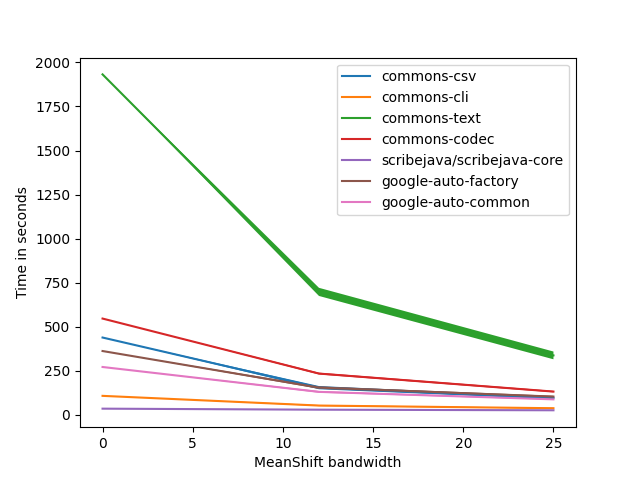
\includegraphics[scale=0.7]{latex_template_thesis_v4-2/meanShiftTime.png}
    \caption{Time over bandwidth for each project}
    \label{fig:my_label}
\end{figure}
\begin{figure}[h!]
    \centering
    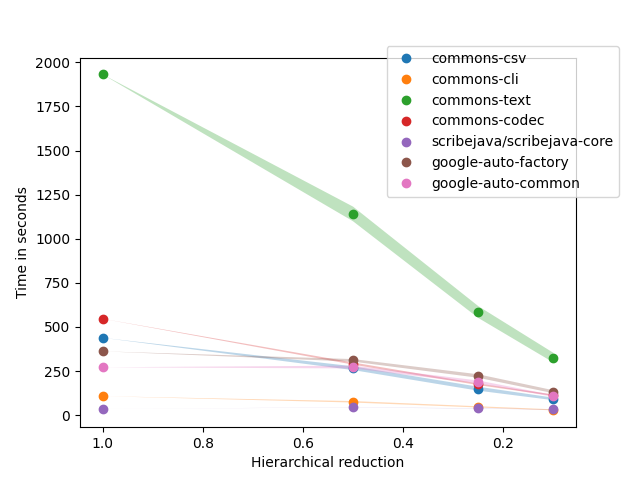
\includegraphics[scale=0.7]{latex_template_thesis_v4-2/hierarchicalTime.png}
    \caption{Time over reduction for each project}
    \label{fig:my_label}
\end{figure}

\clearpage

\section{Discussion}
From the results, we can gather that there is a basis for using clustered mutation testing. An average speedup of 4.5x is significant.
\begin{finding}
Clustered mutation testing can produce a significant speedup.
\end{finding}

It also seems the speedup increases as the number of mutations increases. This can be best observed by comparing the full and 0.1 avg timings of commons-text and scribejava-core. In agglomerative clustering, commons-text goes from 1931.9 to 325.7 seconds. Yet, the smaller project of scribejava-core goes only from 34.9 to 32.1 seconds. This is understandable as the build phase of Pitest for scribejava-core takes up a large part of the mutation testing. This build phase is not reduced by clustered mutation. Alongside this, the supporting algorithms for clustered mutation testing add more time to the entire process than they do for larger projects in a relative sense.
\begin{hypothesis}
The speedup of clustered mutation testing scales with the number of mutants in the project.
\end{hypothesis}

When comparing the speedup of Mean-shift with the speedup of agglomerative clustering, we can see that the differences in speedup are negligible. It would be more reasonable to make a decision between the two based on their performance metrics pertaining to testing capabilities.
\begin{finding}
The differences in speedup between agglomerative and Mean-shift clustering are insignificant on average.
\end{finding}

Closer inspection will however reveal that the Mean-shift clustering outperforms the agglomerative clustering in regards to speedup when it comes to smaller projects, whereas agglomerative clustering seems to be faster for larger projects. Considering bigger projects are more in need of solving the time cost issue of full mutation testing, it would be reasonable to choose agglomerative clustering if a decision were to be made based on speedup.
\begin{hypothesis}
Agglomerative clustering outperforms Mean-shift clustering in terms of speed for larger projects.
\end{hypothesis}

However, the differences in speedup between the two algorithms become smaller as the project size increases in a relative sense. So, while larger projects may see Agglomorative clustering outperform Mean-shift clustering in terms of speed, the choice of the algorithm should still be based on the algorithm's ability to approximate the results of full mutation testing.
\begin{hypothesis}
The differences in speedup between agglomerative and Mean-shift clustering are negligible even for larger projects.
\end{hypothesis}

Considering increasing the reduction has the drawback of decreasing the accuracy of clustered mutation testing, we can not claim that using a reduction of n*0.1 is better than using a reduction of n*0.5. Choosing the reduction or bandwidth is a decision that must be made with the goals of the individual user in mind. Luckily, it is easy to leave this up to the user.

\chapter{Improving CMT by solving presumed weaknesses}
\label{chap:4}
The time analysis has shown us that the number of mutants tested highly influences the speedup. This means a large portion of the time spent during the execution of CMT is spent on the execution of the selected mutants. Consequently, it is unlikely that speeding up the overhead will impact the overall speedup enough for the algorithm to become notably more attractive. Conversely, it also means that we can increase the size of the overhead for the sake of accuracy without losing a significant amount of speedup. In fact, an improvement in accuracy through an increase in the overhead could likely be traded for an improvement in speedup by scaling back the number of mutants tested. These conclusions lead us to the second part of our research: a search for changes in the overhead which increase the accuracy, including ones which have a slightly negative impact on its speed.

There are two design choices in the original CMT algorithm which stood out to us in particular. The first is that the cluster representatives are randomly selected from each cluster. The second is that the data is given mostly raw to the clustering algorithm. In this second part of the research, we will compare two alternative design choices with these two original ones.

\subsection{Center selection}
We will refer to the first alternative design choice as ``center selection''. Here, instead of choosing a random mutant out of each cluster to represent the cluster, we choose the centermost one. Theoretically, the centermost mutant should represent the mutants better than a mutant on the edge of the cluster, as it has more similarity to the other mutants in the cluster on average. To implement this, we have switched over to the ``KMeans'' clustering algorithm, which is comparable to the Agglomerative clustering algorithm in terms of accuracy according to \textcite{Mouissie22}. We did this because Sklearn's KMeans algorithm contains a ``fit\_transform()'' function, which returns the distance of each mutant to each cluster center. This makes it easy to select the mutants with the least distance to their closest cluster center as the representative of that cluster.

\subsection{Pre-processing}
The second alternative design choice is simply more rigorous pre-processing to the same characteristics of the original, as listed in \cref{chap:2}. The only pre-processing the original algorithm did was using label-encoding on all of the categorical identifying characteristics, namely the mutant identifier, return type, class name, and method name. It also used label-encoding on the ID. In the case of nominal data, using label-encoding for clustering causes issues. Consider categorical data that went through label-encoding. One category got encoded to 1, the second to 2 and another one to 8. The clustering algorithm could cluster categories 1 and 2 together, excluding 8. However, in reality, category 2 may not be more similar to category 1 than category 8. The alternative is one-hot-encoding, however, this does increase the overhead to the clustering algorithm as each category gets its own dimension.

Our changed version is composed of multiple steps. First, we encoded the class name, method name and ID using label-encoding just like the original version. ID will keep its label-encoding as the IDs Pitest returns are likely sorted in a way where the label-encoded versions would correctly represent mutant similarity. The method names are also likely to be sorted. Following the label-encoding, the class name and method name are combined with the line number in order to form a new identifying characteristic: ``locality''. This is done by increasing the class name and method name by 100000 and 1000 respectively and adding them to the line number. This way, the clustering algorithm will first separate the mutants by their class name, then their method name and lastly their line number. If the clusters are small enough, mutants from different classes should not be mixed together, thereby solving the issue of label-encoding for class names. If the clusters are not small enough, one-hot-encoding the class name may be preferable. 

Another issue in the original algorithm was that the data was not normalized. Some characteristics had a range in the order of 1, whereas others had a range in the order of 100. This means that some characteristics unintentionally weighed more than others. So, after adding the new numerical characteristics of locality and the now label-encoded ID to the other numerical characteristics we normalized all of them and added weighting. Lastly, the two leftover categorical characteristics, the mutant identifier and return type were added after one-hot-encoding and weighing.

There were several possible approaches to creating fitting weights for each characteristic. The approach chosen for this thesis is the use of the ``fmin'' function from ``Hyperopt''~\cite{Hyperopt}. We decided upon the search spaces by doing smaller runs of Hyperopt and adjusting them accordingly. Sadly, due to hardware failures, we were unable to complete a solid run of the fmin function. So we were left with choosing the best-performing selection from smaller or incomplete runs. This means that the weights chosen for our experiments are but a rough approximation of the optimal weights.

Due to the lack of normalization, it is likely that, in the original algorithm, the ID had the largest impact on how the mutants were clustered, as it had the largest range. In our changed version, ID remains the category with the largest impact, being weighted as such by our crude approximation of the optimal weights. But it has relatively less impact than before, making room for the other characteristics. For example, the impact of locality is about 0.76 of that of ID.

\section{Experiments}
We once again created a Jupyter notebook: ``cmtImprovement.ipynb''~\cite{aAbdalla-repo}. This notebook contains a function which simulates the original CMT algorithm and calculates its precision. The function also contains the option to turn on our new center selection and/or pre-processing changes. If center selection is turned on, the function does not run the algorithm for each given seed, as center selection eliminates the original randomness; it returns the precision of the respective run. Otherwise, it returns all precisions of all seeded runs. As defined in chapter 2, the precision is calculated by dividing the number of correct predictions by the total number of predictions.

For our experiments in the notebook, we ran the original algorithm with the same seeds as \textcite{Basarat21}. We also ran it first with the center selection activated, then with the pre-processing changes activated, and lastly, we ran it with both heuristics activated. We record all returned precisions. The results for each project can be found below. Tables~\ref{tab:05CMT},~\ref{tab:025CMT} and \ref{tab:01CMT} report precisions for all projects and approaches in percentages. The projects are sorted by ascending number of mutants. Alongside these tables, we have created boxplots for all reductions for all projects using PowerBI. For the sake of readability, we have divided the boxplots for each reduction into two.

Lastly, we have created heatmaps comparing the performance of each method to the original. For this, we inserted the samples of the original and the method we wanted to compare into scipy.stats's Mann-Whitney U test~\cite{mannWhitneyU}. If the returned p-value was below 0.05, the precision difference between the original and the compared method can be seen as significant. Otherwise, the difference is insignificant. If the mean precision of the compared method was higher than the mean precision of the original, then the difference is positive. Otherwise, the difference is negative.

For the methods with center selection, however, the comparison can not be done the same way. The p-value returned by the Mann-Whitney U test can be interpreted as the likelihood that the two samples originate from the same underlying distribution. Because center selection causes precisions to be fixed and singular, the Mann-Whitney U test is likely to consider them plausible results of the underlying distribution of the original. Therefore, many of the precision differences between the methods with center selection and the original would be noted as insignificant. 

To solve this, we have defined a significant precision difference differently for the comparison between the center selection methods and the original. We have created a 90\% confidence interval of the mean of the underlying distribution of the original. To achieve this, we have combined the following formula for calculating the percentile value of a random number of the normal distribution:
\[P = \mu + z\sigma\]
Where:
\begin{itemize}
    \item $P$ = Percentile value of a random number of the normal distribution
    \item $\mu$ = Mean of distribution
    \item $z$ = z-score derived from z-table~\cite{ztable}
    \item $\sigma$ = standard deviation of distribution
\end{itemize}
with the central limit theorem, which defines the standard deviation of the means of samples of a normal distribution as:
\[\sigma' = \frac{\sigma}{s}\]
Where:
\begin{itemize}
    \item $\sigma$ = standard deviation of distribution
    \item $s$ = sample size
    \item $\sigma'$ = standard deviation of the means of samples of a normal distribution
\end{itemize}
\[P' = \mu + z\sigma'\]
Where:
\begin{itemize}
    \item $P'$ = Percentile value of the mean of the underlying distribution
    \item $\mu$ = Mean of distribution
    \item $z$ = z-score derived from z-table~\cite{ztable}
    \item $\sigma'$ = standard deviation of the means of samples of a normal distribution
\end{itemize}
We then define an insignificant difference as one within the 90\% confidence interval of the mean of the underlying distribution of the original.

The precision difference between all samples of the methods and all samples of the original, however, does not suffer from the same issue. So the Mann-Whitney U test was still viable for the definition significance for those results. The results of the Mann-Whitney U test on all samples of each method vs all samples of the original are shown in \ref{fig:heatmapAll}.

\section{Results}
\begin{table}[h]
    \centering
    \begin{tabular}{|l|l|l|l|l|l|l|l|}
    \hline
        project & N & original & cs & pp & cs + pp \\ \hline
        google-auto-common & 5219 & 88.7 & 88.7 & 90.2 & 90.4 \\ \hline
        scribejava/scribejava-core & 5746 & 93.8 & 93.8 & 94.4 & 94.4 \\ \hline
        google-auto-factory & 5832 & 92.6 & 92.8 & 93.6 &  93.8 \\ \hline
        commons-csv & 6906 & 90.1 & 89.5 & 91.6 & 91.9 \\ \hline
        commons-cli & 7190 & 87.6 & 87.1 & 89.9 & 90.1 \\ \hline
        google-auto-value & 16746 & 92.1 & 92.0 & 92.6 & 92.8 \\ \hline
        google-gson & 28485 & 90.0 & 89.4 & 91.0 & 91.3 \\ \hline
        commons-io & 44584 & 88.6 & 88.2 & 90.1 & 90.3 \\ \hline
        commons-text & 48490 & 89.7 & 89.4 & 90.7 & 90.7 \\ \hline
        commons-codec & 54804 & 93.6 & 93.4 & 94.8 & 94.8 \\ \hline
    \end{tabular}
    \label{tab:05CMT}
\caption{Mean precisions for 0.5 reduction: original vs center selection vs pre-processing vs both}
\end{table}

\begin{table}[h]
    \centering
    \begin{tabular}{|l|l|l|l|l|l|l|l|}
    \hline
        project & N &original & cs & pp & cs + pp \\ \hline
        google-auto-common & 5219 & 83.6 & 78.2 & 84.8 & 81.8 \\ \hline
        scribejava/scribejava-core & 5746 & 89.7 & 89.6 & 91.7 & 90.6 \\ \hline
        google-auto-factory & 5832 & 89.2 & 85.0 & 90.5 &  89.0 \\ \hline
        commons-csv & 6906 & 86.2 & 81.3 & 86.2 & 84.3 \\ \hline
        commons-cli & 7190 & 83.4 & 76.5 & 83.5 & 81.8 \\ \hline
        google-auto-value & 16746 & 89.1 & 85.6 & 89.3 & 87.7 \\ \hline
        google-gson & 28485 & 85.6 & 83.0 & 86.0 & 84.3 \\ \hline
        commons-io & 44584 & 83.8 & 82.4 & 84.0 & 83.2 \\ \hline
        commons-text & 48490 & 83.8 & 82.7 & 84.7 & 84.3 \\ \hline
        commons-codec & 54804 & 90.4 & 88.8 & 90.9 & 90.4 \\ \hline
    \end{tabular}
    \label{tab:025CMT}
\caption{Mean precisions for 0.25 reduction: original vs center selection vs pre-processing vs both}
\end{table}

\begin{table}[h]
    \centering
    \begin{tabular}{|l|l|l|l|l|l|l|l|}
    \hline
        project & N & original & cs & pp & cs + pp \\ \hline
        google-auto-common & 5219 & 78.6 & 77.7 & 78.1 & 75.8 \\ \hline
        scribejava/scribejava-core & 5746 & 84.7 & 85.4 & 86.7 & 87.6 \\ \hline
        google-auto-factory & 5832 & 86.2 & 85.2 & 85.8 & 86.0 \\ \hline
        commons-csv & 6906 & 82.2 & 79.8 & 82.0 & 81.7 \\ \hline
        commons-cli & 7190 & 78.2 & 77.5 & 78.7 & 77.4 \\ \hline
        google-auto-value & 16746 & 85.0 & 84.0 & 85.0 & 84.2 \\ \hline
        google-gson & 28485 & 79.7 & 80.5 & 79.9 & 80.5 \\ \hline
        commons-io & 44584 & 78.2 & 78.4 & 78.3 & 79.3 \\ \hline
        commons-text & 48490 & 78.9 & 78.6 & 78.7 & 79.1 \\ \hline
        commons-codec & 54804 & 87.2 & 87.4 & 87.6 & 87.5 \\ \hline
    \end{tabular}
    \label{tab:01CMT}
\caption{Mean precisions for 0.1 reduction: original vs center selection vs pre-processing vs both}
\end{table}
\clearpage
\begin{figure}[h!]
    \centering
    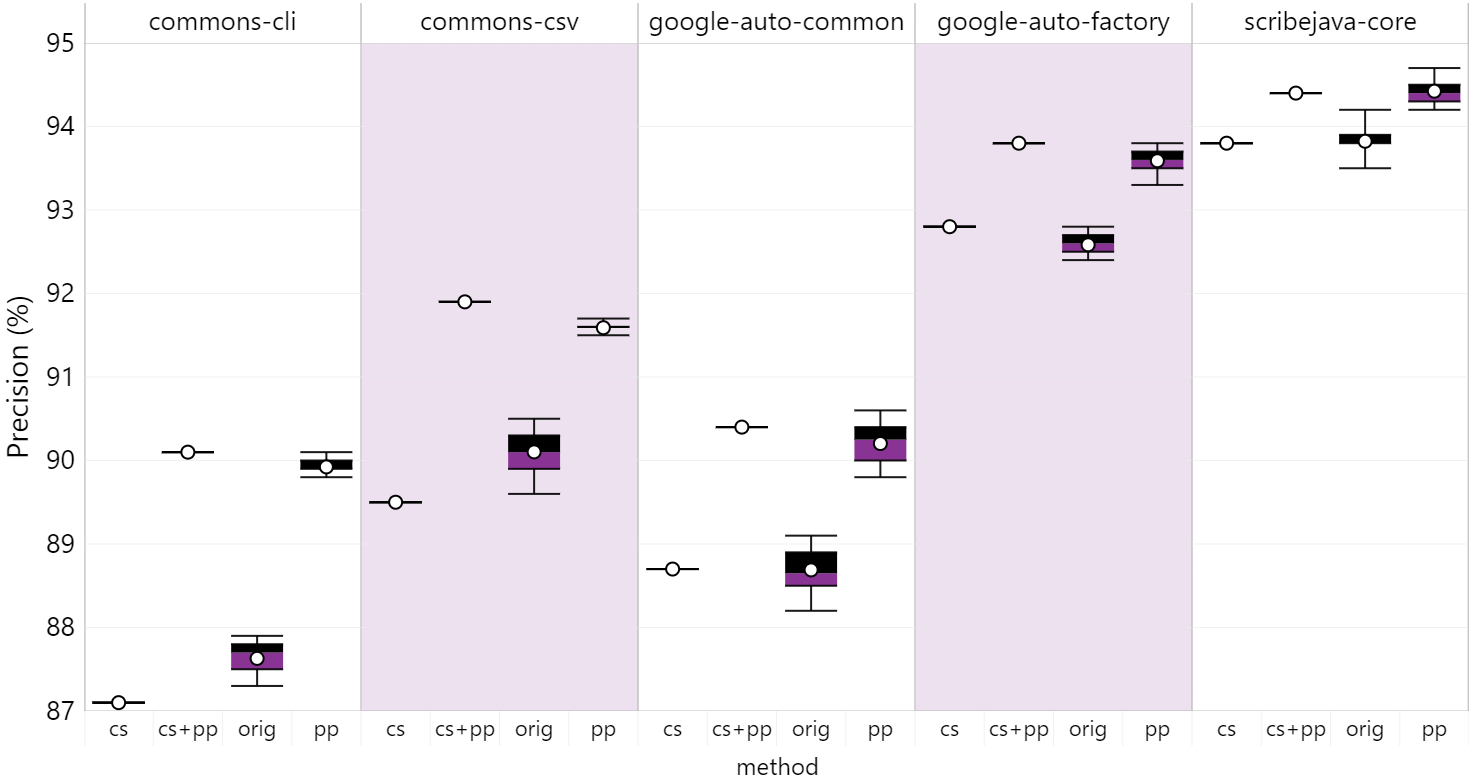
\includegraphics[scale=0.4]{latex_template_thesis_v4-2/05CMTFirst.png}
    \caption{Boxplot of precisions of first batch of projects with reduction: 0.5}
    \label{fig:boxplot05-1}
\end{figure}
\begin{figure}[h!]
    \centering
    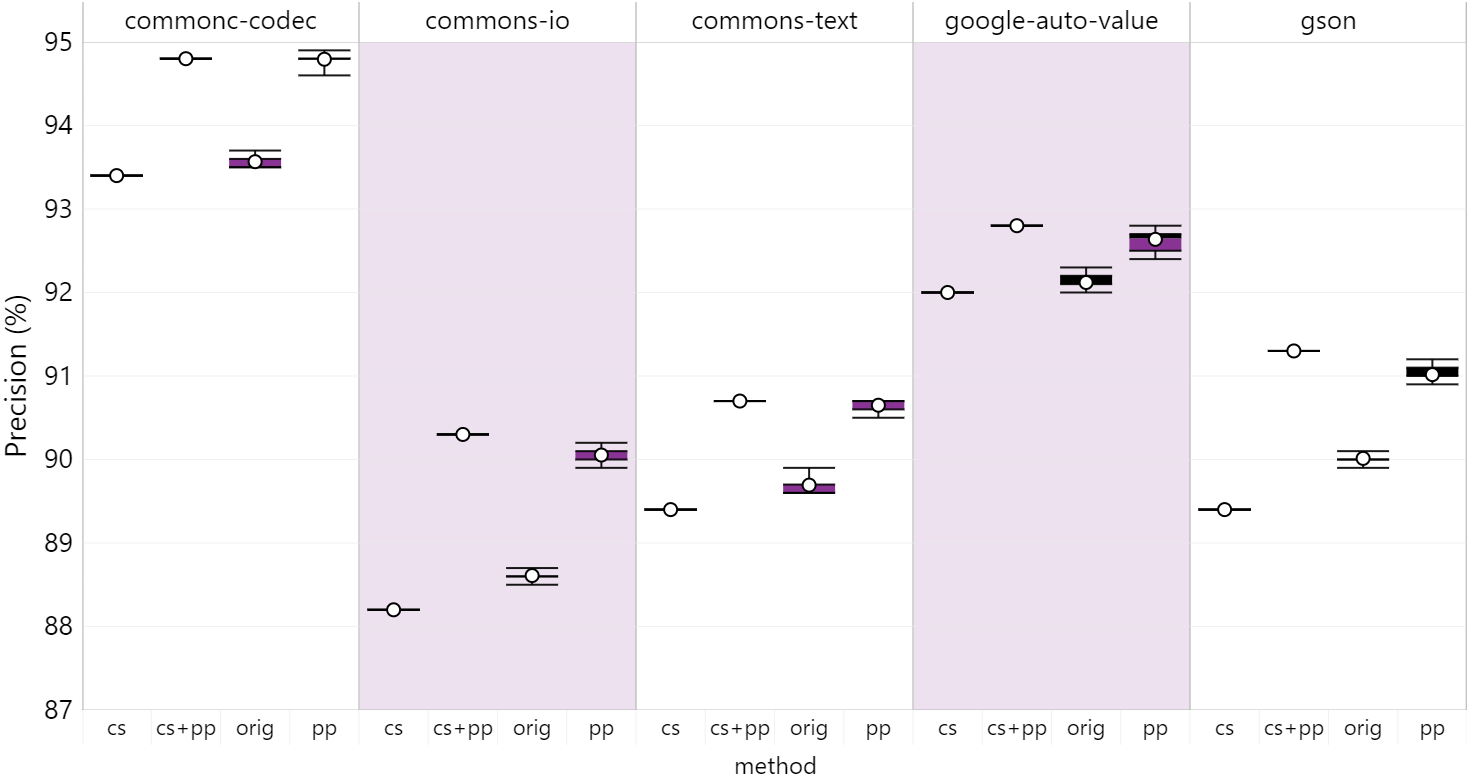
\includegraphics[scale=0.4]{latex_template_thesis_v4-2/05CMTSecond.png}
    \caption{Boxplot of precisions of second batch of projects with reduction: 0.5}
    \label{fig:boxplot05-2}
\end{figure}
\begin{figure}[h!]
    \centering
    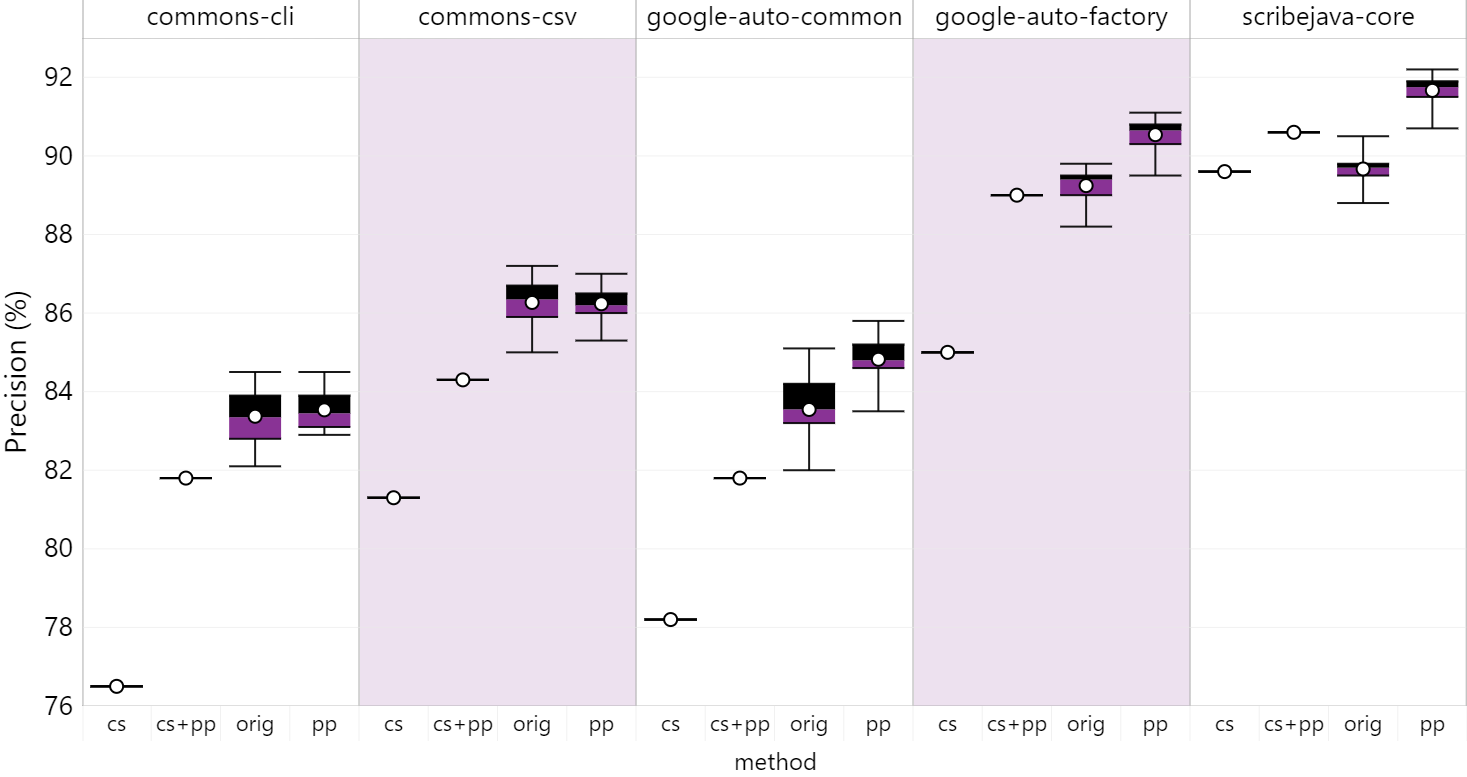
\includegraphics[scale=0.4]{latex_template_thesis_v4-2/025CMTFirst.png}
    \caption{Boxplot of precisions of first batch of projects with reduction: 0.25}
    \label{fig:boxplot025-1}
\end{figure}
\begin{figure}[h!]
    \centering
    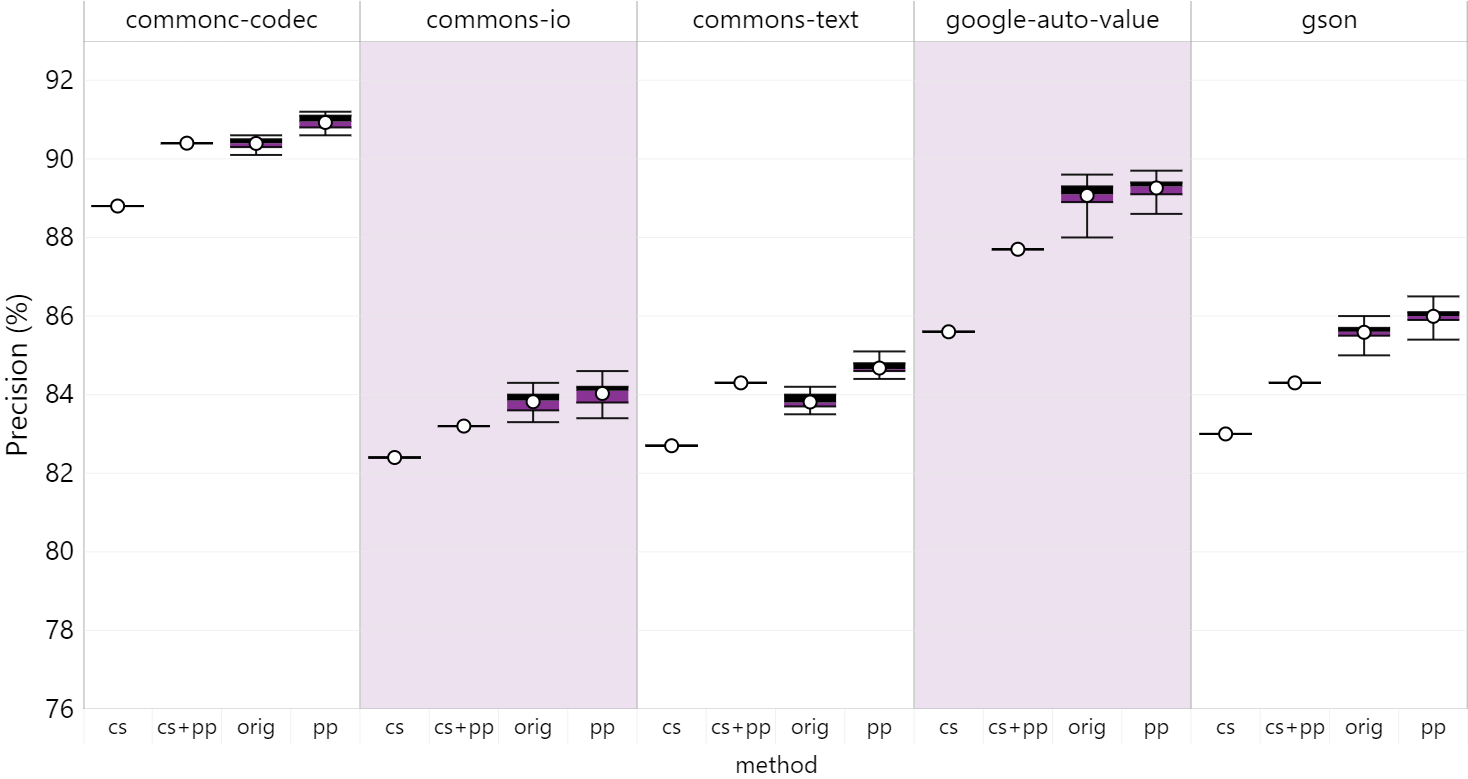
\includegraphics[scale=0.4]{latex_template_thesis_v4-2/025CMTSecond.png}
    \caption{Boxplot of precisions of second batch of projects with reduction: 0.25}
    \label{fig:boxplot025-2}
\end{figure}
\begin{figure}[h!]
    \centering
    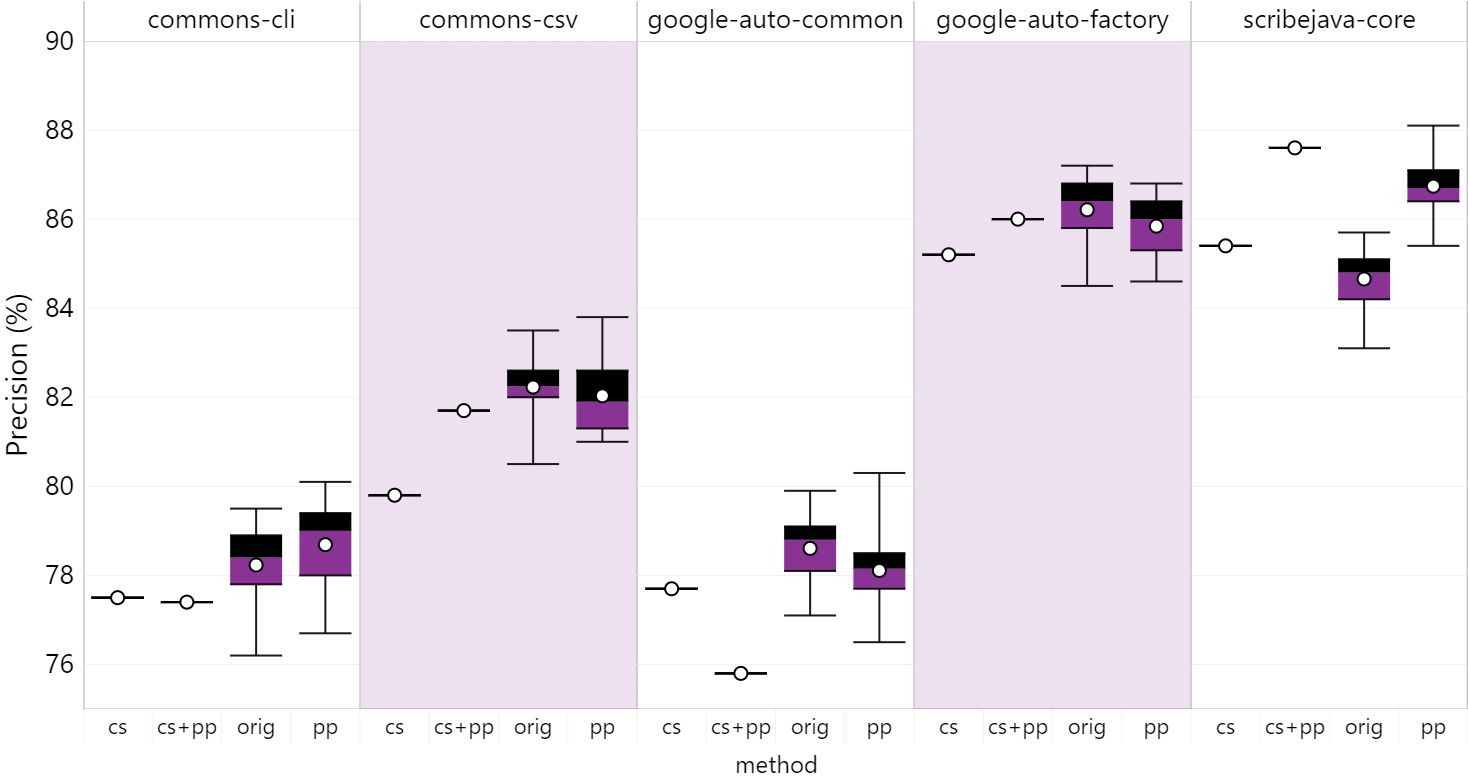
\includegraphics[scale=0.4]{latex_template_thesis_v4-2/01CMTFirst.png}
    \caption{Boxplot of precisions of first batch of projects with reduction: 0.1}
    \label{fig:boxplot01-1}
\end{figure}
\begin{figure}[h!]
    \centering
    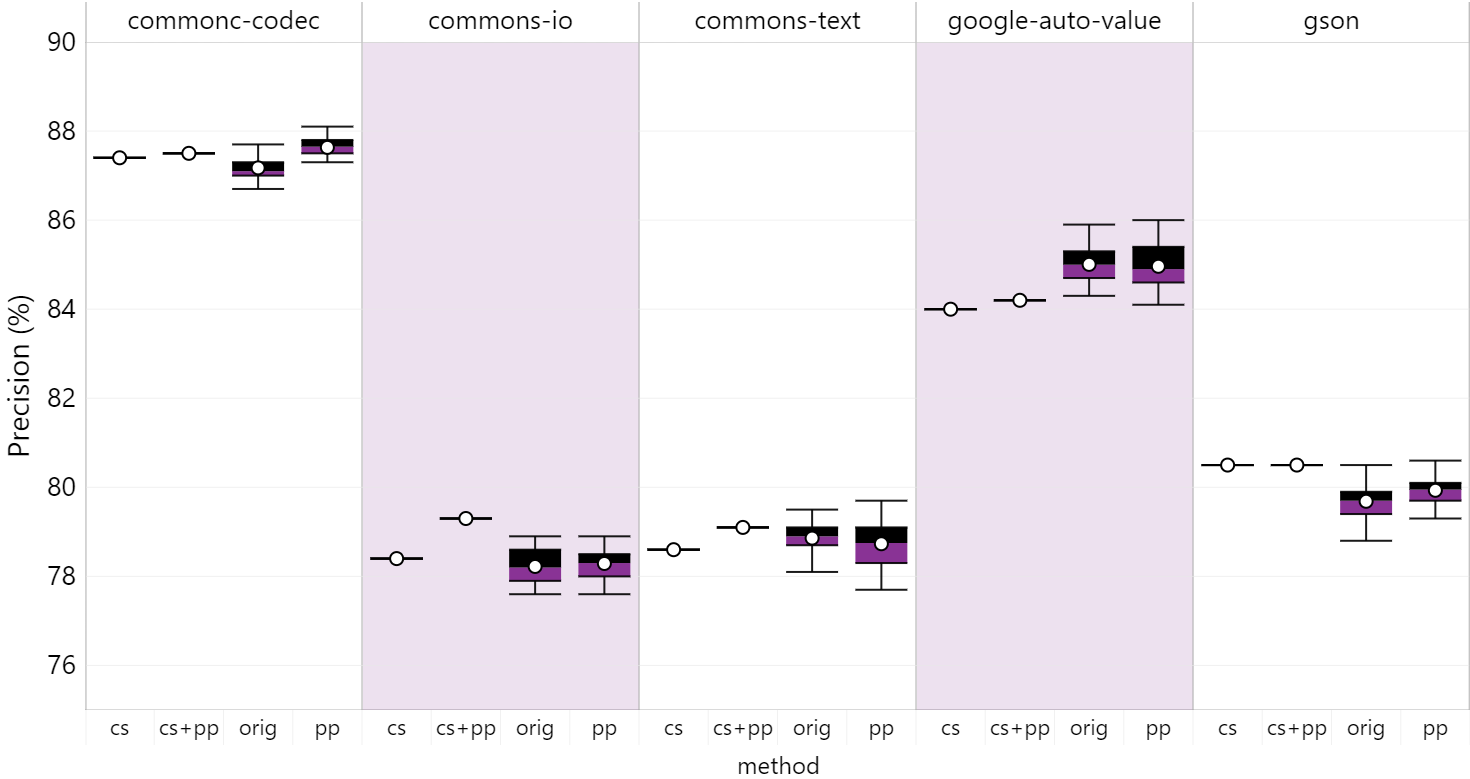
\includegraphics[scale=0.4]{latex_template_thesis_v4-2/01CMTSecond.png}
    \caption{Boxplot of precisions of second batch of projects with reduction: 0.1}
    \label{fig:boxplot01-2}
\end{figure}
\clearpage
\begin{figure}[h!]
    \centering
    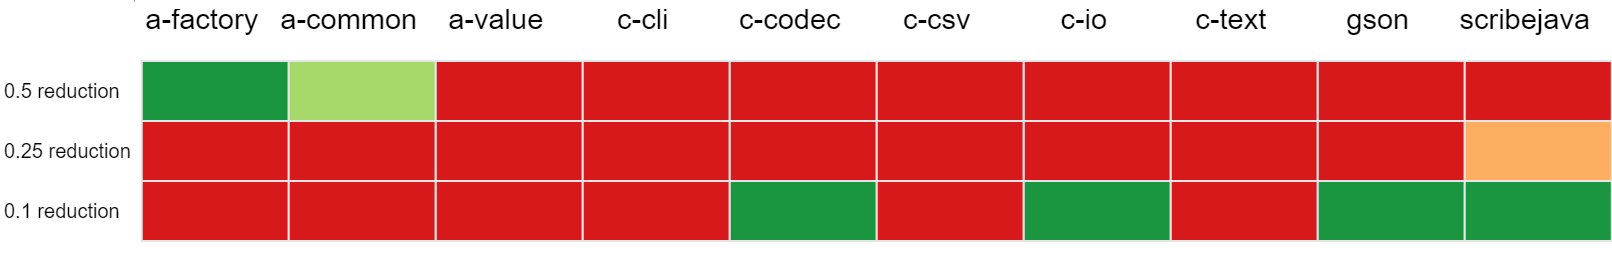
\includegraphics[scale=0.4]{latex_template_thesis_v4-2/csHeatmap.png}
    \caption{Heatmap of center selection vs original regarding precision}
    \label{fig:heatmapCS}
\end{figure}

\begin{figure}[h!]
    \centering
    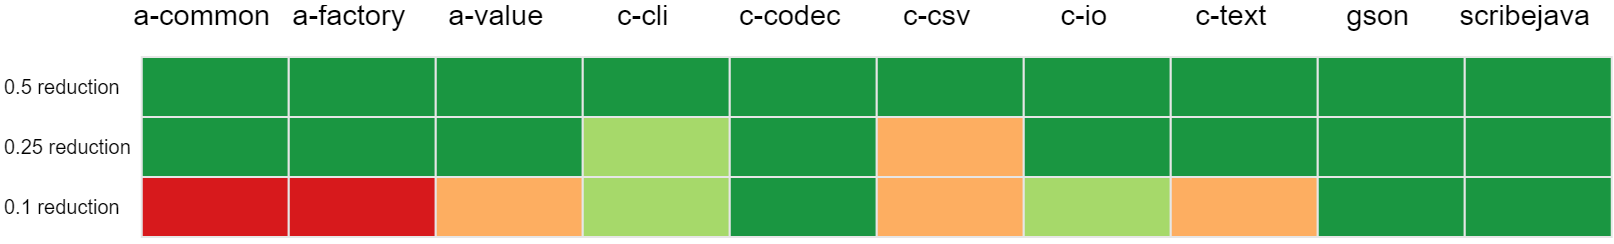
\includegraphics[scale=0.4]{latex_template_thesis_v4-2/ppHeatmap.png}
    \caption{Heatmap of pre-processing vs original regarding precision}
    \label{fig:heatmapPP}
\end{figure}

\begin{figure}[h!]
    \centering
    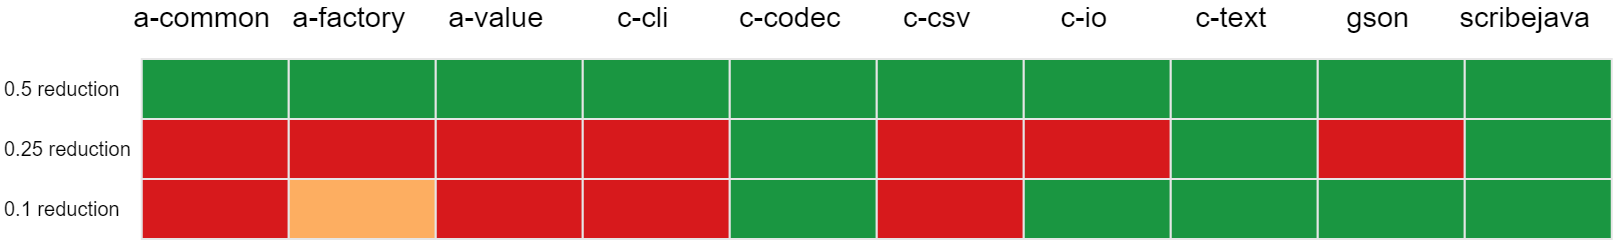
\includegraphics[scale=0.4]{latex_template_thesis_v4-2/csppHeatmap.png}
    \caption{Heatmap of center selection + pre-processing vs original regarding precision}
    \label{fig:heatmapCSPP}
\end{figure}

\begin{figure}[h!]
    \centering
    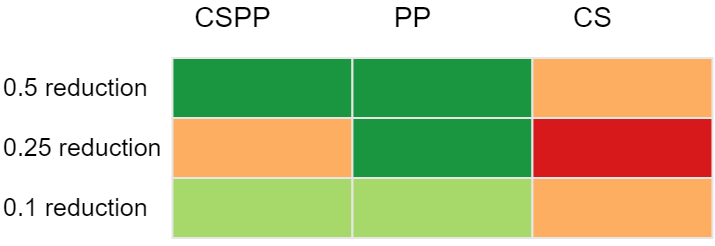
\includegraphics[scale=0.4]{latex_template_thesis_v4-2/allHeatmap.png}
    \caption{Heatmap of all methods vs original regarding precision for all projects}
    \label{fig:heatmapAll}
\end{figure}

\begin{figure}[h!]
    \centering
    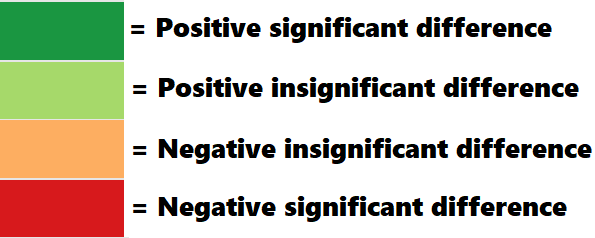
\includegraphics[scale=0.4]{latex_template_thesis_v4-2/heatmapLegend.png}
    \caption{Legend for the above heatmaps}
    \label{fig:heatmapLegend}
\end{figure}



\clearpage
\section{Discussion}
From the more comprehensible figure~\ref{fig:heatmapAll} we can already make a few conclusions. For one, it seems that our more rigorous pre-processing is a beneficial change on average for reduction 0.5 and 0.25. It does get less effective on average when a reduction of 0.1 is chosen. The obvious assumption is that the diversification of the impact characteristics have with pre-processing does not matter as much since clusters are larger and less detailed.
\begin{finding}
    Our pre-processing change is generally a beneficial one at reductions 0.5 and 0.25 for of CMT's precision.
\end{finding}
\begin{hypothesis}
    Our pre-processing change is generally a beneficial one at reduction 0.1.
\end{hypothesis}
A dive into the boxplots shows that the precision increases caused by pre-processing for scribejava-core and commons-codec are not affected by the change in reduction. Although they share the property of being predicted fairly precisely by CMT, google-auto-factory also has this property and does not show the same behavior. The number of mutants in these projects differs largely, so we can also not conclude that this phenomenon is correlated to the size of the project. If more projects are tested and show this behaviour, it might be worth figuring out if we can learn why and take advantage of the underlying reason. It should also be noted that the weighting was done based on the precision of all projects for all tested reductions. Having weighting differ based on the size of the project and reduction may further increase the precision.


Unlike pre-processing, center selection seems to have impacted the precision negatively. A reduction of 0.25 gives a statistically significant precision decrease. But even the other reductions saw the precisions of the tested projects negatively impacted on average. The simplest explanation would be that the centermost mutant is not a worse or better option than others and that this is simply the result of random chance. A more satisfying explanation for this could be that the centermost cluster does not necessarily have the best average similarity with other mutants in the cluster. There could be a sub-cluster within the cluster of which the centermost one is not a part. This would mean that using a different clustering algorithm may see an increase in precision.
\begin{finding}
    Our center selection change is a generally negative change at reduction 0.25 for CMT's precision.
\end{finding}
\begin{hypothesis}
    Our center selection change is a generally negative change at reduction 0.5 and 0.1
\end{hypothesis}
\begin{hypothesis}
    Center selection can perform better when using a different clustering algorithm.
\end{hypothesis}

What is interesting, is that when pre-processing is already on, the addition of center selection actually produced an increase in precision in some cases. The largest project, commons-text turns from an insignificant negative result to a significant positive result. This supports both possible explanations put forward in the previous paragraph, as they could both produce such randomness.

As a whole, we would recommend the addition of pre-processing to the algorithm, perhaps with more rigorous weighting. Even with pre-processing added, it seems that center selection generally creates a slightly negative impact, so we suggest leaving it out in its current form. It does, however, eliminate the randomness sampling creates in the algorithm, which may be desirable when using it multiple times on the same project in a real-world scenario.
\begin{hypothesis}
    Pre-processing is a change beneficial to the precision of CMT, whereas center selection with KMeans is not.
\end{hypothesis}

\chapter{Contextual Predictive Mutation Testing}
\label{chap:5}
In this chapter, we introduce an algorithm which uses a drastically different approach to predict the fate of all mutants using the fate of a selection of tested mutants. The idea behind this approach originates from deliberations made during our search for improvements to the CMT algorithm. Before moving on from CMT with the idea that there was little left to do to improve it, we considered another potential improvement. CMT only bases its prediction on a singular similar mutant. Our first thought was to use the distance to other tested mutants as an indication of similarity and have them impact the prediction as well. The issue is that the scenario in which mutants from multiple entirely different clusters are a better indicator than one from the same cluster would be very rare, if at all possible. But the idea of taking the fate of other similar mutants into account remained appealing. This, combined with the idea of \textcite{Zhang16}, which uses a classifier with each characteristic as a feature, resulted in the algorithm we named ``Contextual Predictive Mutation Testing''.

\section{Creation of the algorithm}
The basic idea is to gather information about a specific project through the execution of a subset of its mutants and then feed that information to a classifier. In other words, the main job of the algorithm is to create a contextual data set for a classifier. The creation of the data set for the training of the classifier is very similar to the creation of the data set for prediction.

First, the algorithm creates the locality feature in the same way as our CMT pre-processing improvement does. It then clusters all continuous data to create categorical data using KMeans1D~\cite{kmeans1d}. With all the characteristic data being categorical, it takes a random, parameter-specified number of mutants from each category for each characteristic, creating the subset of mutants. Afterwards, it executes the entire list. The result of this serves as our source of contextual information. The fates of the mutants in the list are used to calculate what percentage of the mutants are killed from each category for each characteristic, resulting in the pk-score.

An important design decision here was to use the entire list of mutants for every calculation, rather than only the mutants picked specifically for that category. This means that a mutant selected for the sake of calculating the pk-score for a particular category of a characteristic, will also contribute to all other categories it's in for other characteristics. The negative effect of this design choice is that the accuracy of the pk-score for each category will differ across runs and projects. And so the classifier has to deal with features which may differ in their reliability. The positive effect, however, is that the classifier gets fed a lot more information.

For the training set, this process is repeated multiple times, similar to sub-sampling. Doing sub-sampling this way as opposed to simply adding more mutants to the list for calculations is because the latter option creates a difference in the reliability of some features between the training and prediction sets. The amount of sub-sampling can be controlled with a parameter.

With all pk-scores, it replaces each category of each characteristic, in the original, full data set of mutants, with the pk-score, resulting in a new data set. The training and prediction are then executed. In the case of prediction, the predicted results of the executed mutants are retroactively replaced by their actual result.

To choose which classifier to use we selected a few based on Sklearn's algorithm cheat-sheet~\cite{skCheatSheet} and tested them. Since we are predicting a category using labeled data with more than 50 samples, we want to use a classification algorithm according to the cheat-sheet. But we were uncertain as to how many samples would be used in the final algorithm. Therefore, the cheat sheet resulted in the selection of both SGDClassifier and LinearSVC. We also decided to test basic logistic regression. The tests were done loosely as the algorithm parameters were not yet decided upon. The precisions of the classifiers were all very similar, so we chose to continue with LinearSVC, as it was recommended over logistic regression by the cheat sheet and had fewer parameters than SGDClassifier, which would complicate our research. For the parameters of the entire algorithm, we once again attempted a complete, large run of Hyperopt. This was once again thwarted by hardware failure, so we settled for a rough approximation just as for the parameter selection for pre-processing.

We have also coded 3 variations of the algorithm for the sake of deeper analysis. The first variation is simply using 3 projects picked at random from the list excluding the project to be predicted. The original was trained on all 9 projects other than the predicted one. This variation should give us some insight on how much impact increasing or decreasing training sets has on the precision of the classifier. At first, the algorithm used Agglomorative clustering to change the continuous data into categorical data. During our early experiments, we noticed that this part took a long time, so we switched over to KMeans1D. We did notice that the precision was affected by this change, so our second variation is the reintroduction of 3D-Clustering. This should give us some insight into how the pre-processing affects precision. Our last variation replaces the original method of to-be-tested mutant selection with one based on clustering. So the list of mutants to-be-tested is the same list of mutants that gets tested for the center selection variant of CMT.

\section{Experiments}
The entire algorithm was implemented in the notebook ``cpmt.ipynb''~\cite{aAbdalla-repo}. The 3D-Clustering and cluster selection variations have separate notebooks.

The algorithm contains randomness, so the same seeds that have been used throughout this thesis and its predecessors were used. We are focusing on an approximation of a reduction of 0.1 as we believe it to be the most attractive version for commercial use. The precisions are calculated by dividing the number of correct predictions by the total number of predictions. Table~\ref{tab:cpmt} shows the mean precisions for all seeds for each variation for each project in percentages. Figure~\ref{fig:boxplotCPMTPrecisions1} and~\ref{fig:boxplotCPMTPrecisions2} show more detailed precision statistics. The reductions are calculated by dividing the number tested mutants by the total number of mutants in the project. These are visible in figure~\ref{fig:boxplotCPMTReductions1} and~\ref{fig:boxplotCPMTReductions2}. Lastly, we have also kept track of the timings of the overhead of every single run, for this see figure~\ref{fig:boxplotCPMTTimings1} and~\ref{fig:boxplotCPMTTimings2}.

\section{Results}
\begin{table}[h]
    \centering
    \begin{tabular}{|l|l|l|l|l|l|l|l|}
    \hline
        project & N & orig & 3-Proj & 3D-Clus & cs \\ \hline
        google-auto-common & 5219 & 74.6 & 73.1 & 77.2 & 76.5 \\ \hline
        scribejava/scribejava-core & 5746 & 68.9 & 70.5 & 76.8 & 86.9 \\ \hline
        google-auto-factory & 5832 & 83.4 & 81.8 & 79.3 & 82.7 \\ \hline
        commons-csv & 6906 & 85.1 & 85.1 & 85.2 & 75.6 \\ \hline
        commons-cli & 7190 & 80.8 & 80.9 & 81.6 & 76.0 \\ \hline
        google-auto-value & 16746 & 78.7 & 77.8 & 82.9 & 73.0 \\ \hline
        google-gson & 28485 & 71.0 & 70.0 & 69.6 & 81.1 \\ \hline
        commons-io & 44584 & 69.8 & 69.8 & 77.0 & 86.9 \\ \hline
        commons-text & 48490 & 79.4 & 79.2 & 80.6 & 80.7 \\ \hline
        commons-codec & 54804 & 85.2 & 84.7 & 87.2 & 68.0 \\ \hline
    \end{tabular}
    \label{tab:cpmt}
\caption{Mean precisions in percentages of 4 different variations of CPMT.}
\end{table}

\begin{figure}[h!]
    \centering
    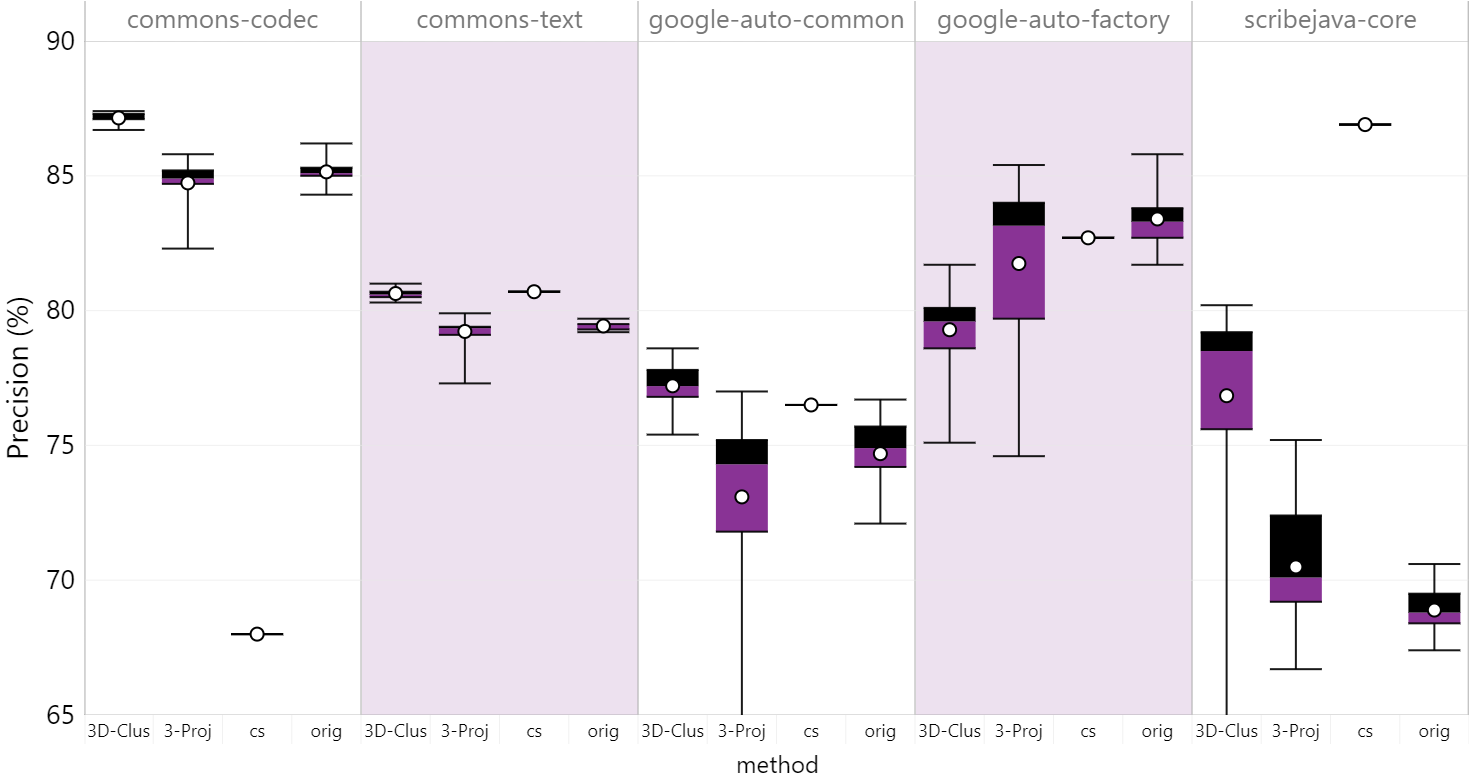
\includegraphics[scale=0.4]{latex_template_thesis_v4-2/PrecisionsCPMTFirst.png}
    \caption{Boxplot of precisions of CPMT for first batch of projects}
    \label{fig:boxplotCPMTPrecisions1}
\end{figure}
\begin{figure}[h!]
    \centering
    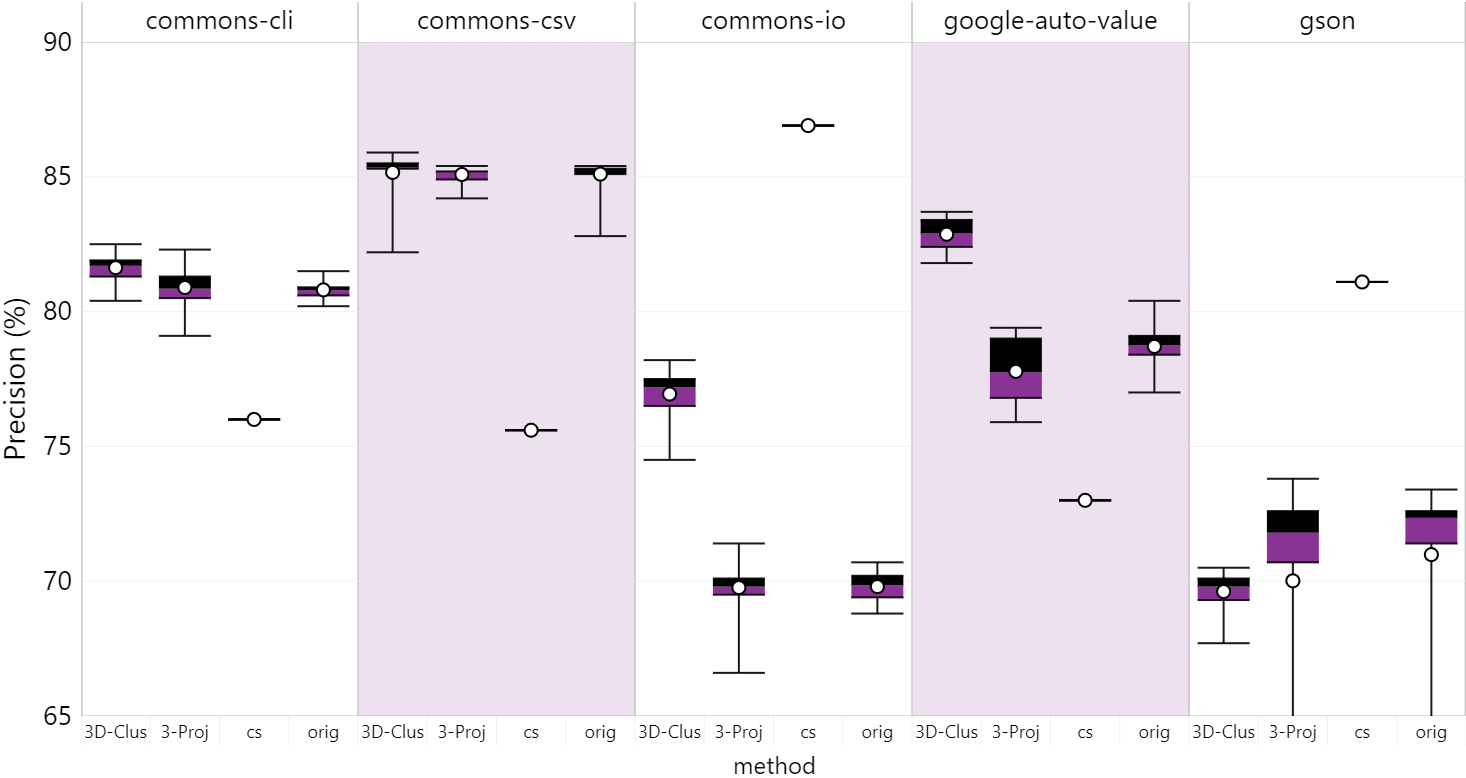
\includegraphics[scale=0.4]{latex_template_thesis_v4-2/PrecisionsCPMTSecond.png}
    \caption{Boxplot of precisions of CPMT for second batch of projects}
    \label{fig:boxplotCPMTPrecisions2}
\end{figure}
\begin{figure}[h!]
    \centering
    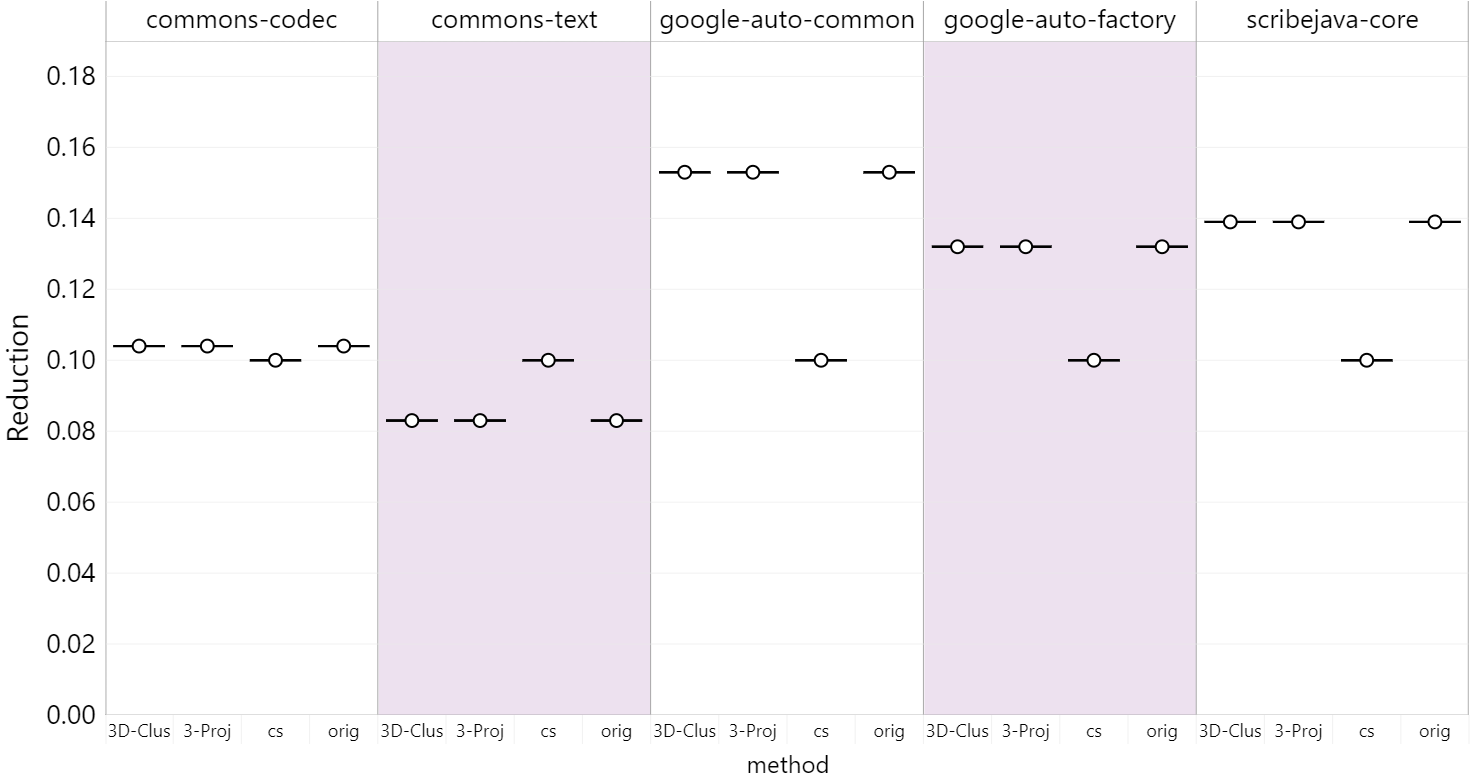
\includegraphics[scale=0.4]{latex_template_thesis_v4-2/ReductionsCPMTFirst.png}
    \caption{Boxplot of reductions of CPMT for first batch of projects}
    \label{fig:boxplotCPMTReductions1}
\end{figure}
\begin{figure}[h!]
    \centering
    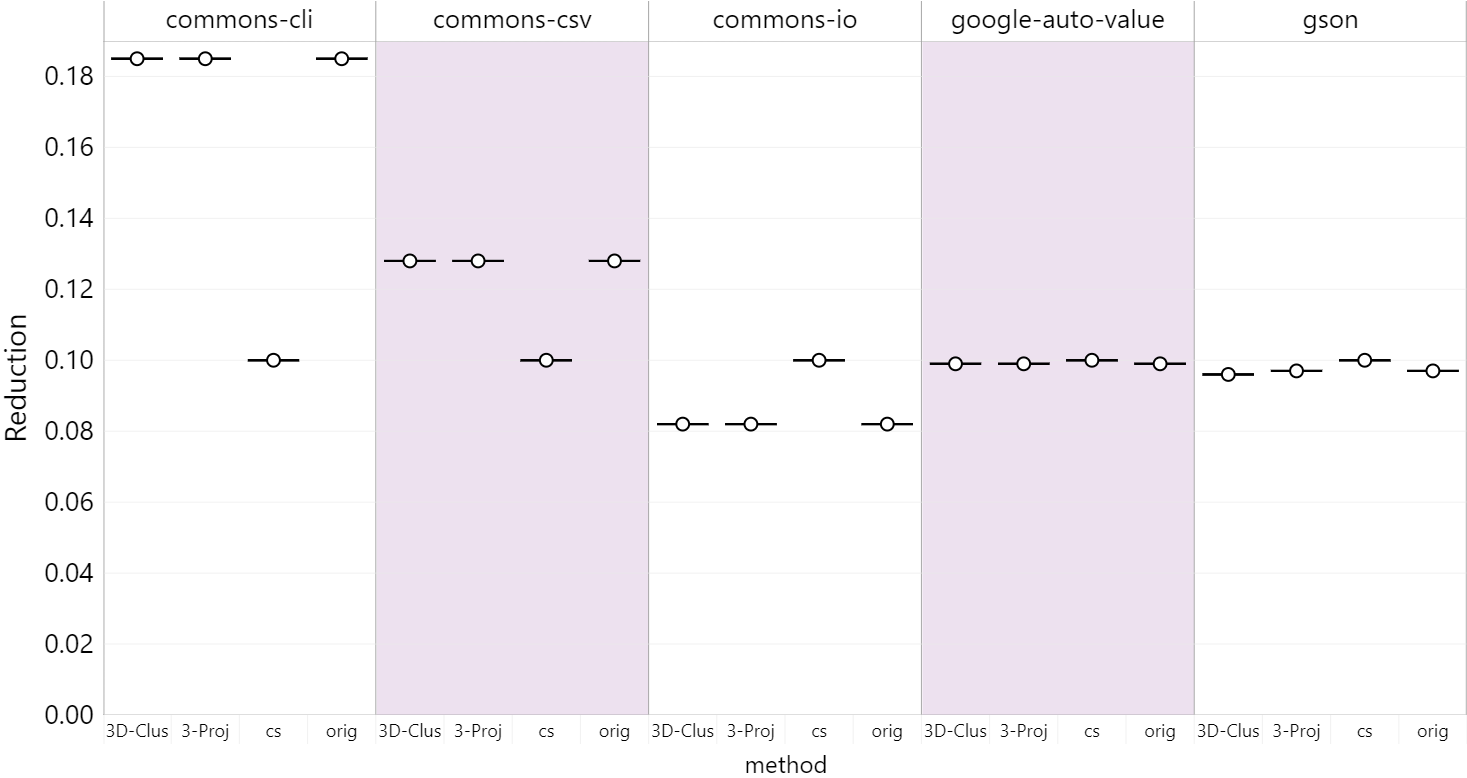
\includegraphics[scale=0.4]{latex_template_thesis_v4-2/ReductionsCPMTSecond.png}
    \caption{Boxplot of reductions of CPMT for second batch of projects}
    \label{fig:boxplotCPMTReductions2}
\end{figure}
\begin{figure}[h!]
    \centering
    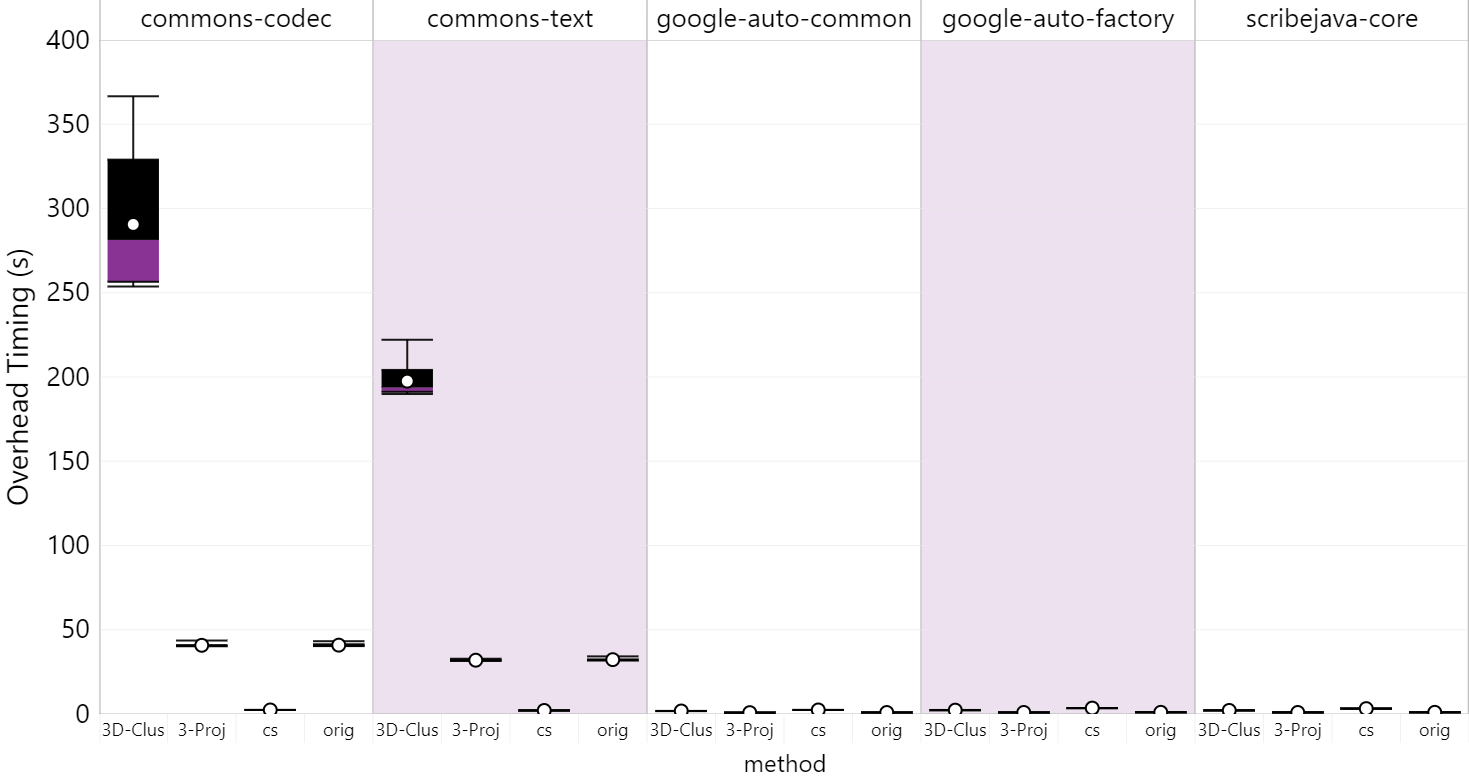
\includegraphics[scale=0.4]{latex_template_thesis_v4-2/TimingsCPMTFirst.png}
    \caption{Boxplot of overhead timings of CPMT for first batch of projects}
    \label{fig:boxplotCPMTTimings1}
\end{figure}
\begin{figure}[h!]
    \centering
    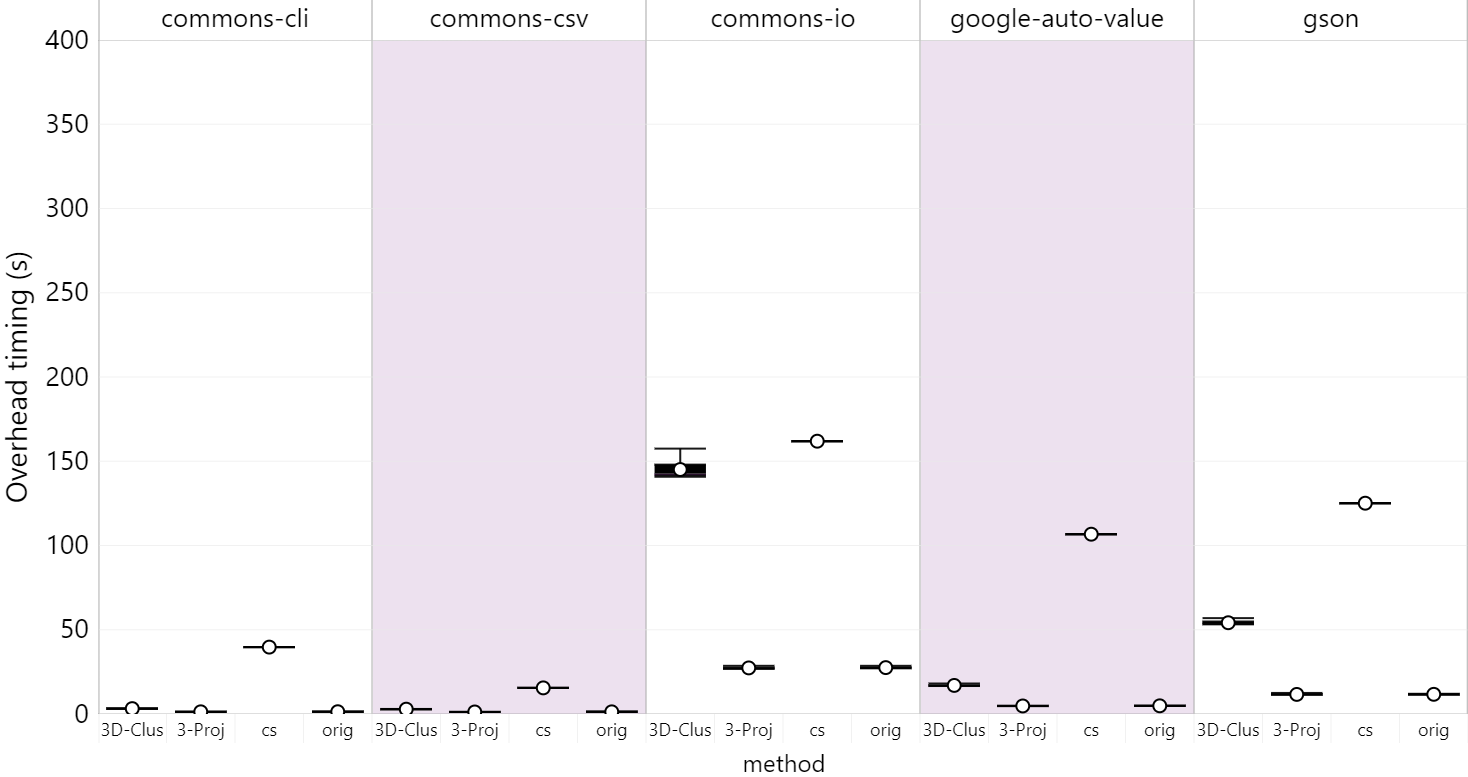
\includegraphics[scale=0.4]{latex_template_thesis_v4-2/TimingsCPMTSecond.png}
    \caption{Boxplot of overhead timings of CPMT for second batch of projects}
    \label{fig:boxplotCPMTTimings2}
\end{figure}

\clearpage

\section{Discussion}
In its current state, the algorithm already seems to be performing pretty well. However, its performances are highly varying. The lowest mean precision calculated is Scribejava-core's 68.89\%. This is surprising, as the precision CMT reaches when predicting Scribejava-core is one of its highest. But we can see that the precision with cluster selection is a much higher 86.9\%. This means that the selection of mutants for the algorithm matters a lot for Scribejava-core. This is further supported by the fact that the 3D-clustering precision results differ by a decent margin from the original. This is despite the fact that the switch to 3D-clustering only affects some of the characteristics of pre-processing. Other cluster selection variants also show drastically different results from their counterparts. As such, we can safely say that the precision of the CPMT algorithm is highly dependent on the selection of the mutants-to-be-tested list.
\begin{finding}
    The precision of the CPMT algorithm is highly dependent on the selection of the mutants-to-be-tested list.
\end{finding}

Although the precisions of the 3D-clustering variant are generally higher than those of the original, figure~\ref{fig:boxplotCPMTTimings1} and~\ref{fig:boxplotCPMTTimings2} show that 3D-clustering also increases the overhead timing a lot, especially for larger projects. So we deem it better to opt for 1D-clustering in the future. Since the continuous data is only in 1 dimension, however, it could also be worth considering a custom partition and categorization of the data.

The reductions are highly variant as well, but this is likely easily changed with a different set of parameters. It does seem that the reductions for larger projects are generally lower, while their precisions are not necessarily lower than their smaller counterparts. Since we are mostly interested in imitating full mutation testing for larger projects, this is a pleasant result.
\begin{hypothesis}
    Reductions of CPMT with the tested set of parameters scale inversely with project size.
\end{hypothesis}

The precisions, as unstable as they are, are promising. It does not yet reach the average precision of CMT with a 0.1 reduction, but it should be noted that there may still be a lot of room left for improvement for this algorithm. But the precisions for some projects do outmatch their CMT counterparts. Regardless of its performance in comparison to other algorithms, the results do prove that basing predictions on multiple mutants is a valid, albeit mayhaps unstable, approach.

The results of training the classifier with 3 projects and the results of training the classifier with 9 projects were also interesting. Training the classifier with only 3 projects caused it to be a lot more unstable. This is likely simply because the projects were picked at random and some projects likely do not provide the classifier with a lot of quality training material. However, the higher ends of the precision results given by the random experiments of 3-projects training coincide with those of the original. This is true for all projects, even those that do not have projects from the same source in the possible training source, like Scribejava-core. So, adding more training than the original has would likely not result in a large increase in precision. At least not with the current algorithm.
\begin{hypothesis}
    Increasing the size of the training set would not improve the classifier's precision significantly.
\end{hypothesis}

Having said that, using a different classifier than the algorithm currently uses may change this. A classifier that can learn more complex patterns may do so when provided with a large training set created by CPMT. One could also look towards availing a neural network as the classifier. However, the number of projects used in our work may be too limited to provide the neural network with enough training data.

The calculation phase of the algorithm is likely even more vital to the results than selection. The current algorithm treats all mutants for each category equally. This means that mutants with more similarity to the mutant that receives the calculated score will have no more impact on that score than others. Of course, more similarity does mean the mutant is used for the calculation of more scores, so the mutant will have more impact on the feature set of the mutant it is more similar to as a whole. Still, this linear increase in impact based on similarity may not be ideal. With CMT showing that the most similar indicator is a powerful predictor, we may want to leverage the similarity of mutants for our calculations. The problem with this is that the current calculation is done per category, whereas a similarity comparison must be done per mutant pairing. So this improvement to the calculation may bring along an undesirable inflation in timing. Perhaps there is a way for similarity to be availed in an acceptable time. Or maybe there is some other improvement to the calculation left to be made.
\begin{hypothesis}
    There are improvements to CPMT's calculation phase yet to be made, which will significantly improve its precision.
\end{hypothesis}

There are also a few simpler potential improvements. A more thorough employment of Hyperopt may lead to a slight improvement in precision, as well as reduction. There is the possibility that a change in the classifier would cause a slight improvement as well. There is also the fact that parameters are currently absolute values. Making them dependent on something like the project size could also be beneficial. If there is a way to accurately predict which variant will perform better, one could also implement a switch between them based on the prediction. After all, where the original algorithm performs badly, center selection seems to perform well and vice versa.

A more meticulous examination of what led to the results than we have presented here could also lead to some ideas for improvements. After all, the precision, timing and reduction are all highly unstable. There were notable precision differences both between variants and projects. It is possible that there is a change that would cause a large improvement that was not revealed by our inspection. 

\chapter{Overall discussion}
\label{chap:6}
\section{Reflecting on results}
For the sake of putting all our results into context, we have noted the mean precisions across all projects of \textcite{Zhang16}'s ``Predictive Mutation Testing'', or ``PMT'' for short.
\begin{table}[h]
    \centering
    \begin{tabular}{|l|l|l|l|l|l|l|l|}
    \hline
      Method & Precision\\ \hline
      PMT: cp & 0.900\\ \hline
      PMT: cv & 0.942\\ \hline
    \end{tabular}
    \caption{\textcite{Zhang16}'s PMT (cross-project and cross-version) precisions}
\end{table}

We have also created 1 more heatmap showing the Mann-Whitney U test on the original CPMT vs CMT with pre-processing turned on:

\begin{figure}[h!]
    \centering
    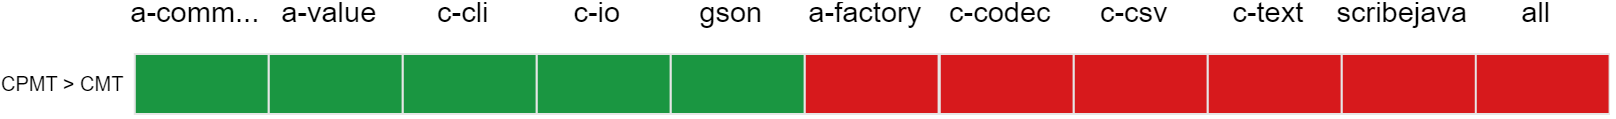
\includegraphics[scale=0.4]{latex_template_thesis_v4-2/cpmtvscmtHeatmap.png}
    \caption{CPMT vs CMT with pre-processing turned on: M-W U test}
    \label{fig:cpmtHeatmap}
\end{figure}

The projects PMT was tested with differed, so these precisions do not serve as an exact comparison. Along with this, the sample size of neither PMT nor CMT/CPMT were enough for a solid indication of standard deviation across projects. But considering the differences in the mean precisions, it is difficult to claim that CMT/CPMT rival PMT in their current forms. Unless a major breakthrough for CMT has been overlooked, the algorithm seems to have reached a limit. The only way for it to possibly be more attractive for commercial use than the state-of-the-art is if a project has not yet been through mutation testing and the user is willing to spend about two-thirds of the time normal mutation testing requires. In our time analysis, we did hypothesise that the speedup may increase for larger projects, but utilizing a reduction of 0.5, the ceiling of its speedup would theoretically be 2x.

CPMT, at least with a reduction of around 0.1, is even less attractive than CMT in the general case. However, as mentioned earlier, the algorithm likely has a lot of room for improvement. Along with this, CPMT actually performed better than CMT for some of the projects. If it can be accurately predicted which algorithm is better for a project, CPMT could already see some practical use in its current form.
\begin{finding}
    With both having a reduction around 0.1, CPMT performs worse than CMT in terms of its ability to approximate the results of full mutation testing in general.
\end{finding}
\begin{finding}
    With both having a reduction around 0.1, CPMT performs better than CMT in terms of its ability to approximate the results of full mutation testing at the same reduction for some projects.
\end{finding}

Another important discussion point is the combination of the algorithms. Both PMT and CPMT can use the same classifiers, whereas CMT results in a single boolean number for each mutant. This means that they can easily be combined into a single feature set to bolster a classifier with more useful information. Of course, combining all three would result in a very large feature set, so the training of the classifier would have to be a lot more extensive. If all three are combined, the selection of the mutants of CPMT could simply be the mutants selected by CMT. Another way they could be combined is through the use of probability. The algorithms may have similar precisions, but perhaps some are more certain about some mutants than others. If this is the case, it can be utilized to increase precision in multiple ways.

Something else that may be of aid to the viability of CMT and even more so CPMT is the usage of C or other lower-level languages. It is highly likely that an algorithm considered for commercial use would be coded in a lower-level language than Python. Considering the speedup this creates for other algorithms, the reduction alone may be a more accurate measurement of speed than the timings reported in this thesis. This assumption would create even more room for more time-complex variants of CMT/CPMT or entirely new algorithms.

\subsection{Answering research questions}
With all our results and deliberation on paper, we turn back to our research questions to see if we have answered them successfully:\\
\textbf{Research question 1:} How does hierarchical clustering mutation testing compare to clusterless mutation testing in terms of speed?\\
\textbf{Research question 2:} How does Mean-shift clustering mutation testing compare to clusterless mutation testing in terms of speed?\\
\textbf{Research question 3:} How can we make improvements to the accuracy performance of clustered mutation testing?\\
\textbf{Research question 4:} How can we create a different algorithm that creates a new avenue for approximating the results mutation testing?\\
Hierarchical CMT creates a speedup over CMT with a range between 1.5x and 4.5x depending on the reduction opted for. Our conjecture is that this speedup would increase with the size of the project, with a hard limit of 1 divided by the reduction. Whether the speedup is worth the cost in precision is dependent on the user's needs. 

Mean-shift CMT showed a similar speedup, at least for the 0.25 and 0.1 reductions. Based on our results, we posited the hypothesis that their similarity in speedup would remain for projects with sizes outside the scope of this thesis.

We have made accuracy improvements to the accuracy of CMT through the use of more rigorous pre-processing. The accuracy improvements were rather small and sadly, our other ideas fell short. Nonetheless, with our discussion surrounding the speed of the overhead in mind, we believe this change to be a clear improvement for CMT.

We can certainly answer question 4 positively with the CPMT algorithm. CPMT is close to CMT in terms of accuracy on average and sometimes even outperforms CMT as a whole for a project. The algorithm is not yet good enough to be presented to the industry, but it has hardly been scrutinized for potential improvements. The algorithm can also contribute to mutation testing through combination with peer algorithms. Of course, the same holds true for CMT.

\section{Ethical aspects of our research}
Our research seeks to speed up and automate the testing of test suites. As such, the ethical questions that arise from our research are the same as the ethical questions surrounding the acceleration and automation of existing tasks in general. Jobs become easier, but some also become at risk of being redundant. Although machines doing our jobs for us sounds pleasant, these developments are prone to being exploited by those in power to increase economic inequalities. Still, we continue our research with the hope that our institutions will ensure that our positive contributions to our field of science do not become negative contributions to society as a whole.

\section{Threats to validity}
\subsection{Time Analysis}
The time analysis was done using only 7 projects. The reason behind this is that all other projects that were tried were either too large, not a green suite, or failed for a different reason. This rendered us unable to solidify the hypotheses made in the chapter into findings. The hypotheses are yet still grounded in good reasoning alongside results, so this should not matter too much.

A smaller issue is that we define the size of the projects by the time it takes to run a full mutation test, but the number of mutants in the project may have been a better indicator of its size.

\subsection{CMT improvements}
The obvious mistake in our CMT improvements is our lack of research on the KMeans algorithm. Although the KMeans algorithm may not be the reason for our disappointing results, the uncertainty could have been prevented.

One of the categorical characteristics was already given in numerical values, the opcode. We did not use one-hot-encoding on this. The fact that the ``perOpcode'' parameter of CPMT had a large influence, whereas the weight of opcode in CMT pre-processing was rather low, indicates that this may have been a mistake. But it does not prove it. Along with this, one-hot-encoding the class name may have also been better than adding it to locality, as discussed before. But these types of pedantic changes are not necessary at this stage of research, as their impact would probably be too insignificant to influence decisions going forward.

\subsection{CPMT}
For the tests of CPMT we wanted to approximate a reduction of 0.1. We had achieved an average reduction of 0.10 through the use of Hyperopt. However, near the end of our work we noticed that the average reduction had jumped to an average of 0.12. We could not find out where this increase came from, nor could we afford to rerun Hyperopt at that stage. Luckily, the larger projects, which we were more interested in, still had a low reduction.

\subsection{Hyperopt}
Of course, not having a solid run of Hyperopt and being forced into a crude approximation of the ideal parameters is a weakness in this thesis. Much like the one-hot-encoding, however, this is likely not going to cause an issue for the future of our research.

\section{Conclusions}
In the first part of our research, we performed a time analysis for clustered mutation testing for the sake of putting the accuracy cost measured by the preceding theses into context. We have done this using the Agglomerative and Mean-shift clustering algorithms which were put forward by \textcite{Basarat21} and \textcite{Mouissie22} respectively. We have found that, for average-sized projects and above, the speedup difference between the two favors Agglomerative clustering by a negligible amount. We have concluded that the choice of clustering algorithm should be made with mainly the accuracy cost in mind, rather than the time cost. We have also found that clustered mutation testing using larger reductions produces a significant speedup. Despite that, the reduction amount should be left up to the user.

The second part of our research focused on the accuracy of CMT. Here, we improved its precision for reductions 0.5 and 0.25 in general and also for reduction 0.1 for the tested projects. We did this by improving its pre-processing. We also attempted to change the selection of mutants for the better, but this ended up negatively impacting its precision. We offered some potential explanations for this, which may lead to better results in future work.

Lastly, we proposed, implemented and tested a novel algorithm we call ``Contextual Predictive Mutation Testing''. The algorithm combines the data set of the characteristics of each mutant with the results of a selection of tested mutants and uses that to predict the other mutants in the project. The algorithm performs slightly worse than CMT, but does outperform it for some projects. A variant of it may outperform both CMT and \textcite{Zhang16}'s PMT in general in the future. To help this along, points of scrutiny which may produce such a variant were discussed. It could also be combined with them, which may result in a better algorithm. 

\section{Future research}
Future research on the time analysis part of clustered mutation testing could be the testing of the hypotheses. One could also seek to further improve the precision of CMT. The CMT overhead code could also be converted to a lower-level language in order to create a time analysis closer to that of a version ready for commercial use.

There exist topics of research which are more likely to be fruitful though. CPMT is more likely to have room for improvement. We discussed this more extensively in the discussion of \cref{chap:5}. CPMT could also be coded into a lower-level language. Since CPMT is more time-complex than CMT, this would give us a better indication of how much more time-complex we can make the overhead before the algorithm becomes undesirable.

A different topic would be the combination of algorithms. While PMT is likely difficult to reproduce, it would be easy to combine CMT and CPMT. The results of this could be game-changing, or very unimpressive.

We also want to mention that there was another algorithm created. The inspiration for it was taken from networks and so we have called it ``Network Mutation Testing'' for now. It was implemented in ``nmt.ipynb''~\cite{aAbdalla-repo}. We abandoned research on the algorithm, as it was lacking in both precision and speed. But that decision was made rather hastily and so it may yet be a first step towards a successful algorithm or a good inspiration for another.

\printbibliography

\appendix

\chapter{Pitest and Pitest clustering plugin}\label{Pitest and Pitest clustering plugin}
\begin{verbatim}
<plugin>
  <groupId>org.Pitest</groupId>
  <artifactId>Pitest-maven</artifactId>
  <version>1.9.8</version>
  <dependencies>
    <dependency>
      <groupId>com.niverhawk</groupId>
      <artifactId>Pitest-clustering-plugin</artifactId>
      <version>1.0-SNAPSHOT</version>
    </dependency>
  </dependencies>
  <configuration>
    <outputFormats>
        <param>HTML</param>
        <param>XML</param>
        <param>CSV</param>
    </outputFormats>
    <exportLineCoverage>true</exportLineCoverage>
    <mutators>
      <mutator>ALL</mutator>
    </mutators>
    <threads>6</threads>
  </configuration>
</plugin>
\end{verbatim}

\chapter{Junit dependency}\label{Junit dependency}
\begin{verbatim}
<dependency>
    <groupId>org.junit.jupiter</groupId>
    <artifactId>junit-jupiter</artifactId>
    <version>5.9.1</version>
    <scope>test</scope>
</dependency>
\end{verbatim}

\end{document}
